\documentclass[9pt,a4paper,twocolumn]{article}

% ------------------------------------------------------------------
% PACKAGES
% ------------------------------------------------------------------
\usepackage[utf8]{inputenc}
\usepackage[T1]{fontenc}
\usepackage{newtxtext}
\usepackage{newtxmath}
\usepackage{geometry}
\usepackage{setspace}
\usepackage{hyperref}
\usepackage{xcolor}
\usepackage{listings}
\usepackage{graphicx}
\usepackage{float}
\usepackage{booktabs}
\usepackage{tabularx}
\usepackage{enumitem}
\usepackage{amsmath}
\usepackage[skip=1.5pt]{caption}
\usepackage{titlesec}
\usepackage{tikz}
\usetikzlibrary{positioning,arrows.meta}
\usepackage{url}

% Image search paths (figures from NEBULA + Postman screenshots)
\graphicspath{{./}{figures/}{imagenes/}}

\setlist{
    noitemsep,
    topsep=0pt,
    partopsep=0pt,
    parsep=0pt
}

\titlespacing*{\section}
{0pt}{5pt}{2pt}

\titlespacing*{\subsection}
{0pt}{4pt}{1.5pt}

\titlespacing*{\subsubsection}
{0pt}{3pt}{1pt}

% ------------------------------------------------------------------
% COLORS
% ------------------------------------------------------------------
\definecolor{PrimaryColor}{HTML}{1A365D}   % Azul oscuro elegante
\definecolor{SecondaryColor}{HTML}{DD6B20} % Naranja vibrante
\definecolor{AccentGreen}{HTML}{2F855A}    % Verde para detalles
\definecolor{CodeBg}{HTML}{F7FAFC}         % Gris muy claro para fondo de codigo
\definecolor{CodeFrame}{HTML}{E2E8F0}      % Gris para el borde del codigo


\newcommand{\REVIEW}[1]{\textcolor{orange}{[Review: #1]}}

% Page configuration
\geometry{margin=1.7cm}
\setlength{\columnsep}{0.7cm}
\onehalfspacing

% Hyperlinks
\hypersetup{
    colorlinks=true,
    linkcolor=black,
    urlcolor=black
}

% Configuracion de bloques de codigo (listings)
\lstset{
    backgroundcolor=\color{CodeBg},
    basicstyle=\ttfamily\small,
    breaklines=true,
    captionpos=b,
    commentstyle=\color{AccentGreen}\itshape,
    keywordstyle=\color{PrimaryColor}\bfseries,
    stringstyle=\color{SecondaryColor},
    frame=single,
    rulecolor=\color{CodeFrame},
    showstringspaces=false,
    xleftmargin=5pt,
    xrightmargin=5pt,
    aboveskip=15pt,
    belowskip=15pt
}

% ------------------------------------------------------------------
% DOCUMENT
% ------------------------------------------------------------------
\begin{document}
\twocolumn[
\begin{center}
    \begin{tabular*}{\textwidth}{@{\extracolsep{\fill}}cc}
        \textbf{Yachay Tech University} &
        \textbf{Web Applications: Workshop Activity 5} \\
        \small School of Mathematical and Computational Sciences &
        \small October 5, 2026
    \end{tabular*}

    \vspace{0.15cm}
    \hrule
    \vspace{0.25cm}

    {\Large\textbf{Building and Testing a REST API with FastAPI, JWT, OpenAPI, and Social Authentication}}

    \vspace{0.1cm}

    {\normalsize Alessa Melo \quad and \quad Freddy Valenzuela}

    \vspace{0.15cm}
    {\normalsize The complete source code of the project is available at \url{https://github.com/Freddyrex/NEBULA_sistema-multiagente}} \\
    \vspace{0.15cm}
    \hrule

    \vspace{0.35cm}
\end{center}
]



\section{General Information}

\begin{itemize}
    \item \textbf{Technology:} Python + FastAPI
    \item \textbf{API Format:} REST/JSON
    \item \textbf{Documentation:} OpenAPI / Swagger UI
    \item \textbf{Authentication:} JWT + OAuth 2.0 social login
    \item \textbf{Testing Tools:} Swagger UI and Postman
    \item \textbf{Database:} SQlite
\end{itemize}

\section{General Objective}

\subsection{Workshop Objective}
\begin{itemize}
    \item Design, implement, document, secure, and test a REST API using FastAPI. The API must provide public and protected endpoints, user registration and authentication
using JSON Web Tokens (JWT), token refresh, logout, a \textit{Remember Me} mechanism, and registration/login using one external social identity provider.
\item Design one or more application-specific entities and implement CRUD operations
protected by JWT authorization.
\end{itemize}

API  has the following structure:

\begin{figure}[H]
\small
\centering
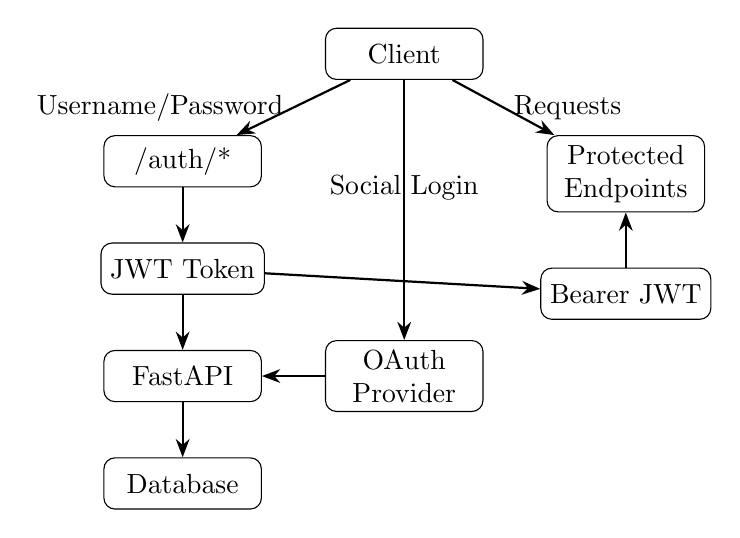
\begin{tikzpicture}[
    node distance=0.7cm and 0.8cm,
    box/.style={
        draw,
        rounded corners,
        align=center,
        minimum width=2cm,
        minimum height=0.65cm
    },
    arrow/.style={-{Stealth}, thick}
]
    \node[box] (client) {Client};
    \node[box, below left=of client] (auth) {/auth/*};
    \node[box, below right=of client] (protected) {Protected\\Endpoints};
    \node[box, below=of auth] (jwt) {JWT Token};
    \node[box, below=of protected] (bearer) {Bearer JWT};
    \node[box, below=of jwt] (fastapi) {FastAPI};
    \node[box, below=of fastapi] (database) {Database};
    \node[box, right=of fastapi] (oauth) {OAuth\\Provider};

    \draw[arrow] (client) -- node[left] {Username/Password} (auth);
    \draw[arrow] (auth) -- (jwt);
    \draw[arrow] (jwt) -- (fastapi);
    \draw[arrow] (client) -- node[right] {Requests} (protected);
    \draw[arrow] (bearer) -- (protected);
    \draw[arrow] (jwt) -- (bearer);
    \draw[arrow] (client) -- node[above] {Social Login} (oauth);
    \draw[arrow] (oauth) -- (fastapi);
    \draw[arrow] (fastapi) -- (database);
\end{tikzpicture}
\caption{General architecture of the FastAPI REST API.}
\label{fig:api_architecture}
\end{figure}

\section{Functional Requirements}
The API must provide the following functionality:
\begin{enumerate}
    \item Public endpoints that can be accessed without authentication.
    \item User registration using a username/email and password.
    \item User login using a username/email and password.
    \item JWT access tokens.
    \item Refresh tokens.
    \item Logout functionality.
    \item \textit{Remember Me} functionality.
    \item A \texttt{/users/me} endpoint.
    \item At least one social authentication provider, such as Google or GitHub.
    \item One or more application-specific entities.
    \item At least one complete CRUD implementation.
    \item JWT-protected endpoints.
    \item JSON request and response bodies.
    \item Automatic OpenAPI documentation.
    \item Testing using Swagger UI.
    \item Testing using Postman.
\end{enumerate}

\section{Project Overview}
The proposed project aims to transform a static Federated Learning (FL) architecture into a dynamic and adaptive system capable of responding to changing conditions in Edge Computing environments. A \textbf{Multi-Agent System (MAS)} will continuously monitor node and network metrics, such as CPU/RAM usage, latency, communication time, and training time, and use a \textbf{Markov Decision Process (MDP)} with Reinforcement Learning to determine appropriate actions. An \textbf{LLM} will complement this process by providing higher-level reasoning for complex or unforeseen situations. The system will be implemented on \textbf{NEBULA}, with modifications to its frontend, controller, and core components to support topology switching between centralized, decentralized, and semi-decentralized configurations, dynamic algorithm selection, and management of slow or unreliable nodes (\textit{stragglers}).

The workshop requirements are fulfilled by a new REST API package added to NEBULA's controller. It provides user registration, JWT access and refresh tokens with rotation, logout, \textit{Remember Me}, Google login, a JWT-protected CRUD for federated-learning experiments, and automatic OpenAPI documentation. It was verified with 22 automated tests (Section~\ref{sec:verification}). Some items still require manual verification and are marked in the text.


\section{Workshop Development}

\subsection{Part 1: Project Preparation}

Since the project is based on the NEBULA\footnote{Official NEBULA repository: \url{https://github.com/CyberDataLab/nebula}} platform, several components required for Federated Learning are already implemented. NEBULA provides a modular architecture composed of a Frontend, Controller, and Core (Figure~\ref{fig:nebula-interface}). The Frontend supports experiment configuration and real-time monitoring, the Controller manages experiment orchestration and node configuration, and the Core executes the federated-learning process on participating devices. NEBULA also provides support for centralized and decentralized architectures, different network topologies, model training, communication between nodes, monitoring, and security mechanisms.

\begin{figure}[H]
    \centering
    \includegraphics[width=0.95\columnwidth,height=5.5cm,keepaspectratio]{figures/Nebula-interface.png}
    \caption{NEBULA application interface for managing federated-learning experiments across participating devices.}
    \label{fig:nebula-interface}
\end{figure}

Therefore, the project does not require the development of the Federated Learning infrastructure from scratch. Instead, the existing NEBULA components were extended with an intelligent orchestration layer (SMAC) and with the authentication and REST API functionality required by the workshop.

The NEBULA environment was configured following the official installation guide and user manual available in the NEBULA documentation~\cite{nebula_docs}. The platform is installed with \texttt{make install}, which uses \texttt{uv} to create a Python~3.11 environment and builds the \texttt{nebula-frontend}, \texttt{nebula-controller} and \texttt{nebula-core} Docker images. It is started with \texttt{python app/main.py}; the web interface is served on port 6060 and the Controller API on port 5050. Instead of the \texttt{requirements.txt} file suggested in the workshop, dependencies are declared in \texttt{pyproject.toml} as dependency groups (\texttt{frontend}, \texttt{controller}, \texttt{core}). The libraries added to the \texttt{controller} group for the REST API are SQLAlchemy~2, \texttt{python-jose[cryptography]} ($\geq$~3.4.0), Authlib, \texttt{httpx}, \texttt{itsdangerous}, \texttt{pydantic[email]} and \texttt{python-dotenv}. The API reuses \texttt{argon2-cffi}, which NEBULA already includes, instead of the \texttt{passlib[bcrypt]} package suggested in the workshop. Other libraries used by the SMAC work are FastAPI~0.114, Uvicorn, Jinja2, aiohttp, aiosqlite, the Groq SDK (with an \texttt{httpx} fallback) and the Firebase JavaScript SDK~10.7.1.

\begin{figure}[H]
    \centering
    \includegraphics[width=0.95\columnwidth,height=5.5cm,keepaspectratio]{nebula_organization.png}
    \caption{NEBULA architecture before the modifications: the Controller launches the nodes and stores the state, and the nodes train peer-to-peer.}
    \label{fig:nebula-organization}
\end{figure}

Figure~\ref{fig:web-home} shows the running web interface (\texttt{http://127.0.0.1:6060/platform}) used for the browser tests of Sections~\ref{sec:verification} and Part~25: the home page with access to Login, registration and Dashboard.

\begin{figure}[H]
    \centering
    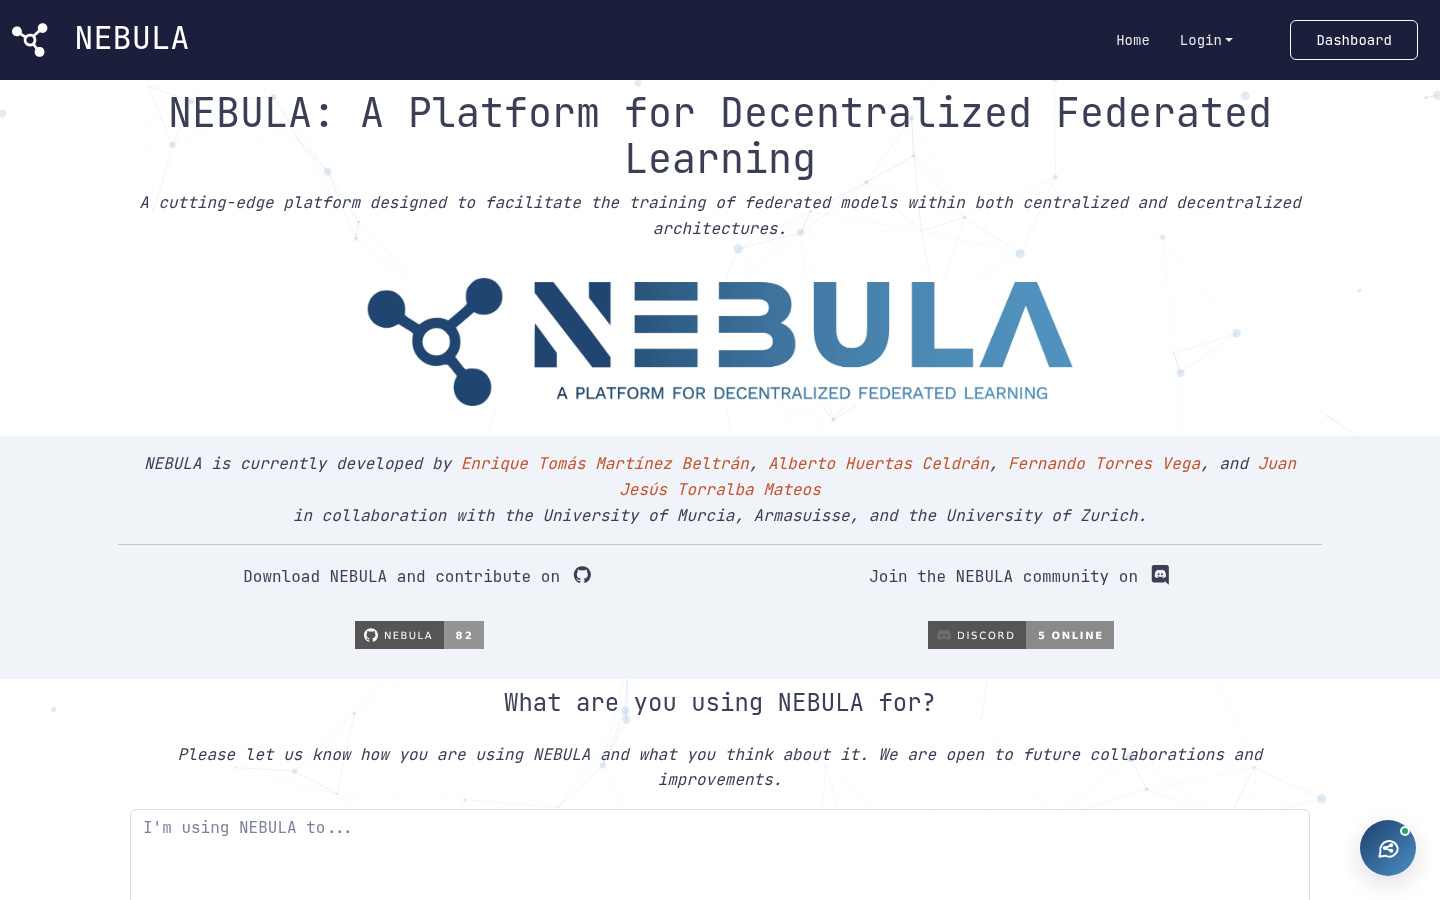
\includegraphics[width=0.95\columnwidth,height=5.5cm,keepaspectratio]{imagenes/01_web_home.png}
    \caption{\footnotesize NEBULA web interface home page running on port 6060.}
    \label{fig:web-home}
\end{figure}

% ------------------------------------------------------------
\subsection{Part 2: API Organization}

The workshop proposes an \texttt{app/} package with \texttt{models/}, \texttt{schemas/}, \texttt{routers/} and \texttt{security/} folders. In NEBULA, the \texttt{app/} folder contains the deployer, not a web application. Therefore the REST API was created as a new package, \texttt{nebula/controller/api/}, which keeps the same four-folder organization. Table~\ref{tab:file-map} lists the new and modified files. All paths are relative to the \texttt{nebula/} folder, except the tests and the project configuration files.

\begin{table*}[t]
\centering
\small
\begin{tabularx}{\textwidth}{>{\raggedright\arraybackslash}X l >{\raggedright\arraybackslash}X}
\hline
\textbf{Location} & \textbf{Status} & \textbf{Purpose} \\
\hline
\multicolumn{3}{l}{\textit{REST API of the workshop}} \\
\texttt{controller/api/\_\_init\_\_.py} & New & \texttt{include\_api()} registers middleware and routers; \texttt{init\_api()} creates the tables; OpenAPI tags \\
\texttt{controller/api/standalone.py} & New & Independent FastAPI application (title, description, version) for Swagger UI and Postman \\
\texttt{controller/api/settings.py}, \texttt{database.py}, \texttt{catalog.py} & New & Environment configuration, SQLAlchemy engine and session, catalog of datasets, models, aggregators and topologies \\
\texttt{controller/api/models/} & New & \texttt{User}, \texttt{RefreshToken}, \texttt{Experiment} \\
\texttt{controller/api/schemas/} & New & Pydantic request and response models \\
\texttt{controller/api/security/} & New & \texttt{passwords.py} (Argon2id), \texttt{jwt.py} (tokens), \texttt{deps.py} (\texttt{get\_current\_user}) \\
\texttt{controller/api/routers/} & New & \texttt{public.py}, \texttt{auth.py}, \texttt{social.py}, \texttt{users.py}, \texttt{experiments.py} \\
\texttt{controller/controller.py} & Modified & Three lines: import, \texttt{init\_api()} in the lifespan, \texttt{include\_api(app)} \\
\texttt{tests/test\_api\_workshop5.py} & New & 22 automated tests \\
\texttt{pyproject.toml}, \texttt{.gitignore}, \texttt{.env.example} & Modified/New & Controller dependencies; \texttt{.env} and \texttt{app/databases/*.db*} excluded from Git; template without real values \\
\hline
\multicolumn{3}{l}{\textit{SMAC orchestration layer}} \\
\texttt{frontend/app.py} & Modified & Registration form, Firebase login, SMAC and metrics endpoints \\
\texttt{frontend/smac\_api.py}, \texttt{smac\_chat.py}, \texttt{metrics/} & New & SMAC endpoints, chatbot backend, TensorBoard metrics \\
\texttt{frontend/templates/}, \texttt{static/js/} & New/Modified & Sign-up page, SMAC control panel, floating chat, Firebase SDK in \texttt{layout.html} \\
\texttt{controller/scenarios.py} & Modified & Adds SMAC agent settings to node configurations \\
\texttt{core/operatorbus.py}, \texttt{smac\_groq.py}, \texttt{pb/nebula.proto} & New/Modified & Command channel to the nodes, Groq client, \texttt{NegotiationMessage} \\
\texttt{core/situationalawareness/awareness/} & New/Modified & Straggler predictor, aggregation selector, resource broker, LLM agent, negotiation \\
\hline
\end{tabularx}
\caption{New and modified files of the current implementation.}
\label{tab:file-map}
\end{table*}
% ------------------------------------------------------------
\subsection{Part 3: FastAPI Configuration}

The REST API is not a separate server by default. NEBULA's Controller already creates a FastAPI application, \texttt{app = FastAPI(lifespan=lifespan)} in \texttt{controller/controller.py}, and the API is attached to it with three added lines:

\begin{lstlisting}[language=Python, basicstyle=\ttfamily\footnotesize]
from nebula.controller.api import \
    include_api, init_api
...
    await initialize_databases(databases_dir)
    init_api()   # create API tables
...
app = FastAPI(lifespan=lifespan)
include_api(app)  # /public /auth /users
                  # /experiments
\end{lstlisting}

The new routes are \texttt{/public/*}, \texttt{/auth/*}, \texttt{/users/me} and \texttt{/experiments}. They do not conflict with the Controller's existing routes (\texttt{/scenarios}, \texttt{/nodes}, \texttt{/notes}, \texttt{/user/...}, \texttt{/physical}). The combined documentation is available at \texttt{http://localhost:5050/docs}.

For development, testing and evaluation, the package also provides an independent application, \texttt{standalone.py}, with \texttt{title="NEBULA API"}, a description, version \texttt{1.0.0} and the list of tags. It is started with:

\begin{lstlisting}[basicstyle=\ttfamily\footnotesize]
uvicorn nebula.controller.api.standalone:app \
    --reload --port 8000
\end{lstlisting}

Its Swagger UI (\texttt{http://127.0.0.1:8000/docs}) shows only the API of the workshop. The tables are created automatically at startup. The frontend application (port 6060) is not modified by the REST API.

% ------------------------------------------------------------
\subsection{Part 4: OpenAPI Documentation}

FastAPI generates the OpenAPI specification automatically (\texttt{/docs} and \texttt{/openapi.json}). Every route of the new API declares a \texttt{tags} group (\textit{Public}, \textit{Authentication}, \textit{Social authentication}, \textit{Users}, \textit{Experiments}), a \texttt{summary}, a \texttt{description}, a \texttt{response\_model} when it returns a body, the \texttt{status\_code} of success and a \texttt{responses} entry for each documented error. Request bodies are Pydantic models with examples, so Swagger UI shows each field, its type and its constraints. The existing NEBULA routes (for example the SMAC endpoints of the frontend) are not part of this documentation and remain under the \textit{default} group.

% ------------------------------------------------------------
\subsection{Part 5: Database}

The project uses two databases that do not interfere with each other.

\paragraph{NEBULA's existing databases.} NEBULA uses SQLite, split into four files stored in \texttt{app/databases/} (configured with \texttt{NEBULA\_DATABASES\_DIR}) and accessed with raw SQL through \texttt{aiosqlite} and \texttt{sqlite3}, without an ORM. The schema is defined in \texttt{nebula/controller/database.py}. All columns are of type \texttt{TEXT}, and the tables are linked logically, without foreign keys (Table~\ref{tab:db-overview}). These files are used by the NEBULA web interface and are not modified.

\begin{table}[H]
\centering
\scriptsize
\begin{tabularx}{\columnwidth}{l l l X}
\hline
\textbf{File} & \textbf{Table} & \textbf{Primary key} & \textbf{Logical relationship} \\
\hline
\texttt{users.db}     & \texttt{users}     & \texttt{user}     & --- \\
\texttt{scenarios.db} & \texttt{scenarios} & \texttt{name}     & \texttt{username} $\rightarrow$ \texttt{users.user} \\
\texttt{nodes.db}     & \texttt{nodes}     & \texttt{uid}      & \texttt{scenario} $\rightarrow$ \texttt{scenarios.name} \\
\texttt{notes.db}     & \texttt{notes}     & \texttt{scenario} & \texttt{scenario} $\rightarrow$ \texttt{scenarios.name} \\
\hline
\end{tabularx}
\caption{NEBULA database files and tables.}
\label{tab:db-overview}
\end{table}

The \texttt{users} table of \texttt{users.db} is limited to authentication and role information (Table~\ref{tab:db-users}). Node-specific information is stored separately in the \texttt{nodes} table (Table~\ref{tab:db-nodes}), which associates each node with a scenario, while the \texttt{scenarios} table (Table~\ref{tab:db-scenarios}) contains the configuration of the federated-learning scenarios.

\begin{table}[H]
\centering
\footnotesize
\begin{tabularx}{\columnwidth}{l l X}
\hline
\textbf{Column} & \textbf{Key} & \textbf{Description} \\
\hline
\texttt{user}     & PK & Username, stored in upper case \\
\texttt{password} &    & Argon2 password hash \\
\texttt{role}     &    & \texttt{admin}, \texttt{user} or \texttt{demo} \\
\hline
\end{tabularx}
\caption{Table \texttt{users} of \texttt{users.db}.}
\label{tab:db-users}
\end{table}

\begin{table}[H]
\scriptsize
\begin{tabularx}{\columnwidth}{l l X}
\hline
\textbf{Column} & \textbf{Key} & \textbf{Description} \\
\hline
\texttt{uid}        & PK & Unique node identifier \\
\texttt{idx}        &    & Node index in the scenario \\
\texttt{ip}, \texttt{port} & & Network address of the node \\
\texttt{role}       &    & Node role (trainer, aggregator, server, \ldots) \\
\texttt{neighbors}  &    & Connected neighbor addresses \\
\texttt{latitude}, \texttt{longitude} & & Node location \\
\texttt{timestamp}  &    & Time of the last status report \\
\texttt{federation} &    & Federation type (CFL, DFL, SDFL) \\
\texttt{round}      &    & Current training round \\
\texttt{scenario}   &    & Scenario the node belongs to \\
\texttt{hash}       &    & Hash of the node state \\
\texttt{malicious}  &    & Whether the node is malicious \\
\hline
\end{tabularx}
\caption{Table \texttt{nodes}.}
\label{tab:db-nodes}
\end{table}

\begin{table}[H]
\centering
\scriptsize
\begin{tabularx}{\columnwidth}{l X}
\hline
\textbf{Group} & \textbf{Columns} \\
\hline
Identification & \texttt{name} (PK), \texttt{title}, \texttt{description}, \texttt{username}, \texttt{role}, \texttt{status}, \texttt{start\_time}, \texttt{end\_time} \\
Deployment & \texttt{deployment}, \texttt{federation}, \texttt{accelerator}, \texttt{gpu\_id}, \texttt{network\_subnet}, \texttt{network\_gateway}, \texttt{logginglevel}, \texttt{report\_status\_data\_queue} \\
Topology & \texttt{topology}, \texttt{nodes}, \texttt{nodes\_graph}, \texttt{n\_nodes}, \texttt{matrix}, \texttt{random\_topology\_probability} \\
Data and model & \texttt{dataset}, \texttt{iid}, \texttt{partition\_selection}, \texttt{partition\_parameter}, \texttt{model} \\
Training & \texttt{agg\_algorithm}, \texttt{rounds}, \texttt{epochs} \\
Security & \texttt{attack\_params}, \texttt{reputation} \\
Mobility & \texttt{random\_geo}, \texttt{latitude}, \texttt{longitude}, \texttt{mobility}, \texttt{mobility\_type}, \texttt{radius\_federation}, \texttt{scheme\_mobility}, \texttt{round\_frequency}, \texttt{mobile\_participants\_percent}, \texttt{additional\_participants}, \texttt{schema\_additional\_participants} \\
\hline
\end{tabularx}
\caption{Table \texttt{scenarios} (44 columns, grouped by purpose).}
\label{tab:db-scenarios}
\end{table}

In addition to the scenario configuration, NEBULA maintains a separate \texttt{notes} table (Table~\ref{tab:db-notes}) for user-written notes associated with each scenario.

\begin{table}[H]
\centering
\scriptsize
\begin{tabularx}{\columnwidth}{l l X}
\hline
\textbf{Column} & \textbf{Key} & \textbf{Description} \\
\hline
\texttt{scenario}       & PK & Scenario name \\
\texttt{scenario\_notes} &   & Free-text notes written by the user \\
\hline
\end{tabularx}
\caption{Table \texttt{notes}.}
\label{tab:db-notes}
\end{table}

\paragraph{Database of the REST API.} The API has its own database, \texttt{api.db}, stored by default in \texttt{app/databases/}. It is accessed through SQLAlchemy~2.0 with real foreign keys, and the tables are created automatically at startup. The \texttt{DATABASE\_URL} environment variable replaces it with MySQL/MariaDB or PostgreSQL without code changes (this was not tested; see Section~\ref{sec:verification}). Tables~\ref{tab:api-users}, \ref{tab:api-refresh} and \ref{tab:api-experiments} describe its structure.

\begin{table}[H]
\centering
\scriptsize
\begin{tabularx}{\columnwidth}{l l X}
\hline
\textbf{Column} & \textbf{Key} & \textbf{Description} \\
\hline
\texttt{id}               & PK & Integer identifier \\
\texttt{username}         & UQ & Up to 150 characters (an email is used for social accounts) \\
\texttt{email}            & UQ & Stored in lower case \\
\texttt{full\_name}       &    & Full name \\
\texttt{password\_hash}   &    & Argon2id hash; \texttt{NULL} for social accounts \\
\texttt{is\_active}       &    & Disabled accounts cannot log in \\
\texttt{role}             &    & \texttt{user} (default) or \texttt{admin} \\
\texttt{auth\_provider}, \texttt{provider\_user\_id} & UQ & \texttt{local} or \texttt{google}; unique together \\
\texttt{created\_at}, \texttt{last\_login} & & UTC timestamps \\
\hline
\end{tabularx}
\caption{Table \texttt{users} of \texttt{api.db}.}
\label{tab:api-users}
\end{table}

\begin{table}[H]
\centering
\scriptsize
\begin{tabularx}{\columnwidth}{l l X}
\hline
\textbf{Column} & \textbf{Key} & \textbf{Description} \\
\hline
\texttt{id}          & PK &  \\
\texttt{user\_id}    & FK & $\rightarrow$ \texttt{users.id}, deleted in cascade \\
\texttt{jti}         & UQ & Unique identifier of the token \\
\texttt{token\_hash} & UQ & SHA-256 of the refresh token (the token itself is never stored) \\
\texttt{remember\_me} &   & Lifetime chosen at login, kept when the token is rotated \\
\texttt{expires\_at}, \texttt{revoked\_at}, \texttt{created\_at} & & Expiration, revocation and creation times \\
\hline
\end{tabularx}
\caption{Table \texttt{refresh\_tokens} (one row per session).}
\label{tab:api-refresh}
\end{table}

\begin{table}[H]
\centering
\scriptsize
\begin{tabularx}{\columnwidth}{l l X}
\hline
\textbf{Column} & \textbf{Key} & \textbf{Description} \\
\hline
\texttt{id}          & PK &  \\
\texttt{user\_id}    & FK & Owner, $\rightarrow$ \texttt{users.id}, deleted in cascade \\
\texttt{name}, \texttt{description} & & Name (up to 100 characters) and free text \\
\texttt{federation}  &    & \texttt{DFL}, \texttt{SDFL} or \texttt{CFL} \\
\texttt{topology}    &    & \texttt{Fully}, \texttt{Ring}, \texttt{Star} or \texttt{Random} \\
\texttt{dataset}, \texttt{model} & & Valid pair according to the NEBULA catalog \\
\texttt{agg\_algorithm} &  & \texttt{FedAvg}, \texttt{Krum}, \texttt{Median} or \texttt{TrimmedMean} \\
\texttt{n\_nodes}, \texttt{rounds}, \texttt{epochs} & & Integers with limits (2--50, 1--1000, 1--100) \\
\texttt{status}      &    & \texttt{draft}, \texttt{queued}, \texttt{running}, \texttt{finished}, \texttt{failed} \\
\texttt{created\_at}, \texttt{updated\_at} & & UTC timestamps \\
\hline
\end{tabularx}
\caption{Table \texttt{experiments}.}
\label{tab:api-experiments}
\end{table}

\paragraph{SMAC files.} The SMAC functionality does not add tables; its operational and audit information is stored in JSON files (Table~\ref{tab:db-files}).

\begin{table}[H]
\centering
\scriptsize
\begin{tabularx}{\columnwidth}{>{\raggedright\arraybackslash}X
                                >{\raggedright\arraybackslash}X}
\hline
\textbf{File} & \textbf{Fields} \\
\hline
\path{app/logs/<scenario>/smac_audit.jsonl} &
\path{ts, user, event, payload} \\

\path{app/logs/<scenario>/smac_decisions.jsonl} &
\path{timestamp, round, owner, action, command_type, priority, confidence, explanation} \\

\path{app/config/<scenario>/operator_commands/<id>.json} &
\path{id, target, action, params, issued_by, issued_at, ttl_s} \\
\hline
\end{tabularx}
\caption{JSON files used by the SMAC features.}
\label{tab:db-files}
\end{table}

% ------------------------------------------------------------
\subsection{Part 6: User Model}

The API user model is the \texttt{User} class of \texttt{controller/api/models/user.py} (SQLAlchemy~2.0, Table~\ref{tab:api-users}). It contains all the fields required by the workshop (\texttt{id}, \texttt{username}, \texttt{full\_name}, \texttt{email}, \texttt{password\_hash}, \texttt{is\_active}, \texttt{created\_at}, \texttt{auth\_provider}, \texttt{provider\_user\_id}) and the optional \texttt{role} and \texttt{last\_login}. A uniqueness constraint on (\texttt{auth\_provider}, \texttt{provider\_user\_id}) prevents duplicate social identities, and \texttt{password\_hash} may be \texttt{NULL} for social-only accounts.

Two decisions differ from the workshop's example. The \texttt{username} column accepts 150 characters instead of 50, because social accounts use their email as username and an email can exceed 50 characters. Timestamps are stored as UTC without time zone, since SQLite does not keep it.

The model is independent from NEBULA's \texttt{users} table (Table~\ref{tab:db-users}), which keeps only a username, an Argon2 hash and a role. NEBULA's table is not modified, so the existing web login keeps working. The consequence is that accounts of the web interface and accounts of the REST API are separate.

% ------------------------------------------------------------
\subsection{Part 7: Registration}

Registration is implemented by \texttt{POST /auth/register}, which receives and returns JSON. The request is validated by the \texttt{UserRegister} schema:

\begin{itemize}
    \item \texttt{username}: 3 to 50 characters; letters, digits, \texttt{\_}, \texttt{.} and \texttt{-}.
    \item \texttt{full\_name}: 1 to 150 characters.
    \item \texttt{email}: valid address (\texttt{EmailStr}).
    \item \texttt{password}: 8 to 128 characters.
\end{itemize}

\begin{lstlisting}[basicstyle=\ttfamily\footnotesize]
POST /auth/register
Content-Type: application/json

{"username": "student01",
 "full_name": "Ana Torres",
 "email": "ana@example.com",
 "password": "MySecurePassword123!"}
\end{lstlisting}

The handler lower-cases the email, checks that neither the username nor the email exist, hashes the password with Argon2id (\texttt{argon2-cffi}) and inserts the user with role \texttt{user} and \texttt{auth\_provider = local}. If two simultaneous requests pass the check, the database uniqueness constraint rejects the second one and it is also answered with 409. The plain-text password is never stored, and the response (\texttt{UserResponse}) does not contain the hash. Table~\ref{tab:register-responses} summarizes the responses.

\begin{table}[H]
\centering
\small
\begin{tabularx}{\columnwidth}{>{\raggedright\arraybackslash}X
                                >{\raggedright\arraybackslash}X}
\hline
\textbf{Case} & \textbf{HTTP response} \\
\hline
Account created & 201 Created \\
Username or email already registered & 409 Conflict \\
Invalid email, short password, invalid username or missing field & 422 Unprocessable Content \\
\hline
\end{tabularx}
\caption{Responses of \texttt{POST /auth/register}.}
\label{tab:register-responses}
\end{table}

The NEBULA web interface keeps its own sign-up form (\texttt{POST /platform/register}, \texttt{register.html}). It uses HTML form data, requests only a username and a password, redirects instead of returning JSON, and writes to NEBULA's \texttt{users.db}. It is part of the web application and not of the REST API. The Postman evidence for this endpoint is shown in Figs.~\ref{fig:postman-register-body} and \ref{fig:postman-register-respuesta}.

The web registration was also tested in the browser: Fig.~\ref{fig:web-register-form} shows the sign-up form (which additionally offers \textit{Sign in with Google} via Firebase), Fig.~\ref{fig:web-register-filled} the filled form, and Fig.~\ref{fig:web-register-result} the home page after the account was created.

\begin{figure}[H]
    \centering
    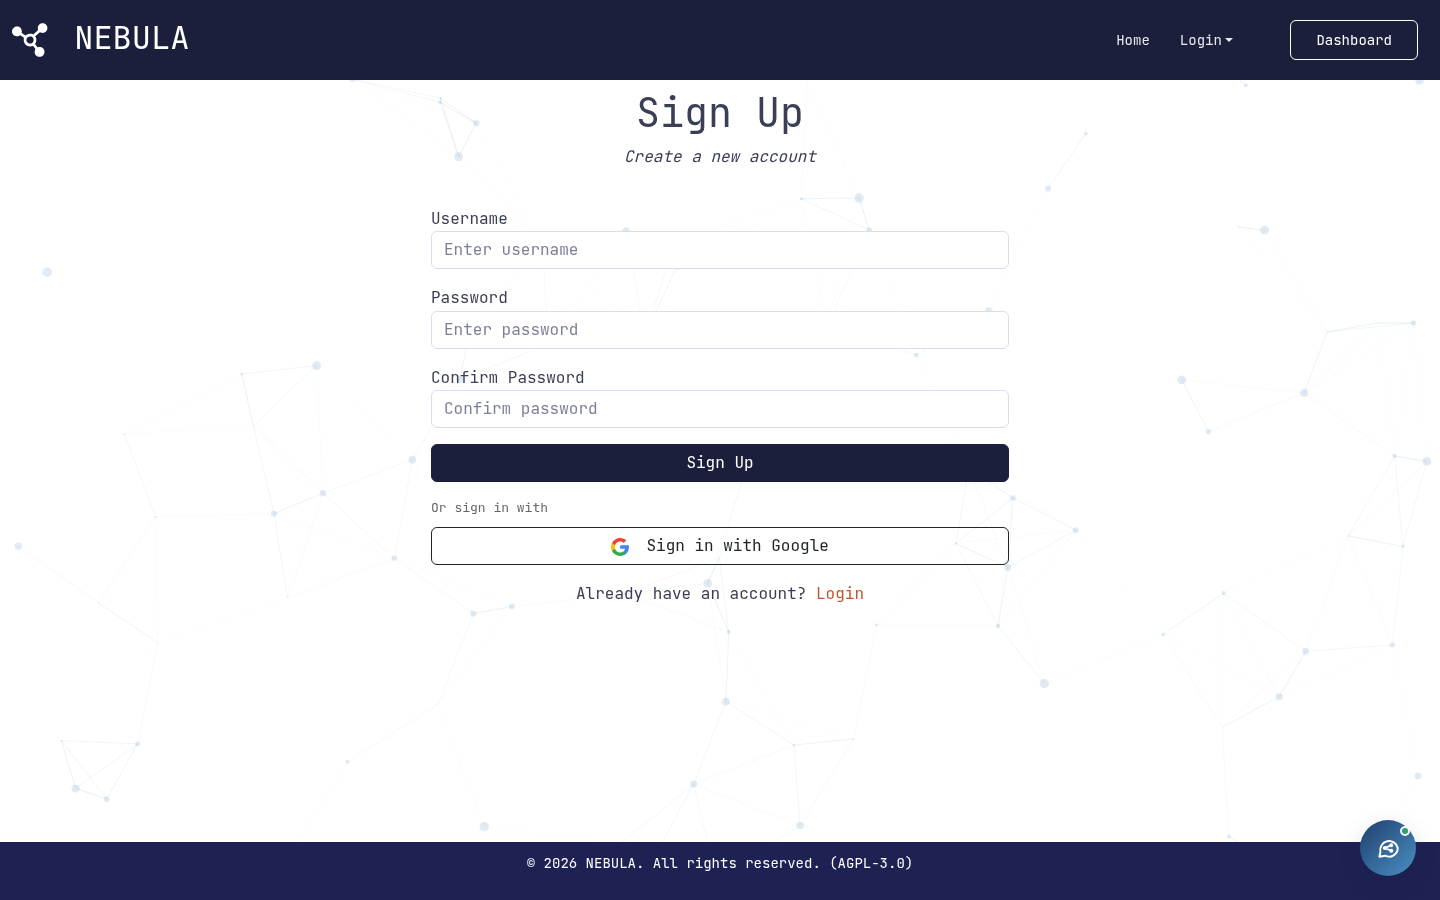
\includegraphics[width=0.95\columnwidth,height=5.5cm,keepaspectratio]{imagenes/02_web_register_form.png}
    \caption{\footnotesize Web sign-up form at \texttt{/platform/register} with username, password and Google options.}
    \label{fig:web-register-form}
\end{figure}

\begin{figure}[H]
    \centering
    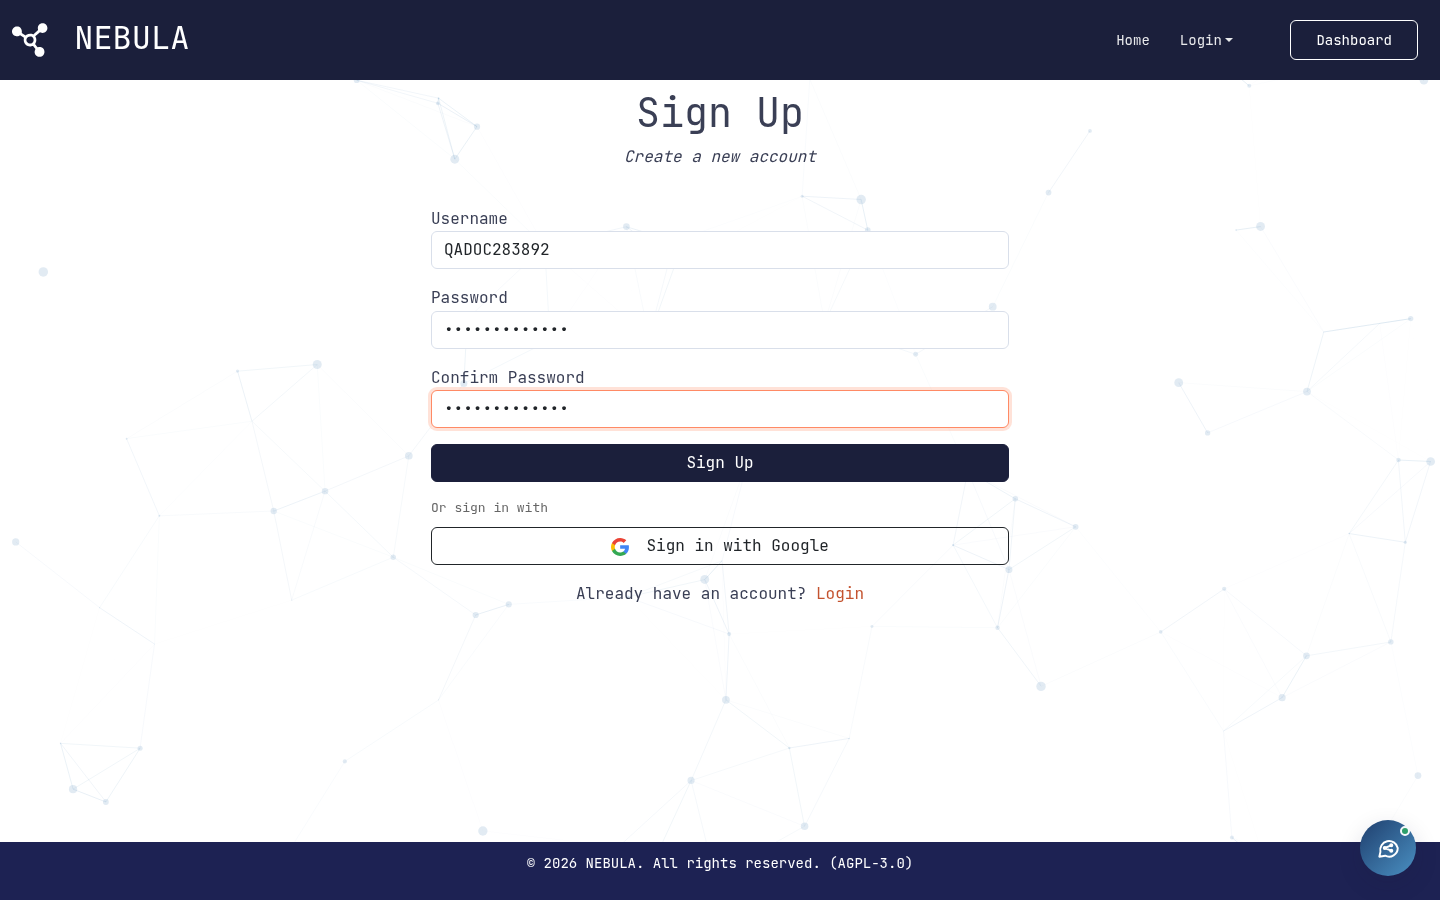
\includegraphics[width=0.95\columnwidth,height=5.5cm,keepaspectratio]{imagenes/03_web_register_filled.png}
    \caption{\footnotesize Web sign-up form filled with the QA account data.}
    \label{fig:web-register-filled}
\end{figure}

\begin{figure}[H]
    \centering
    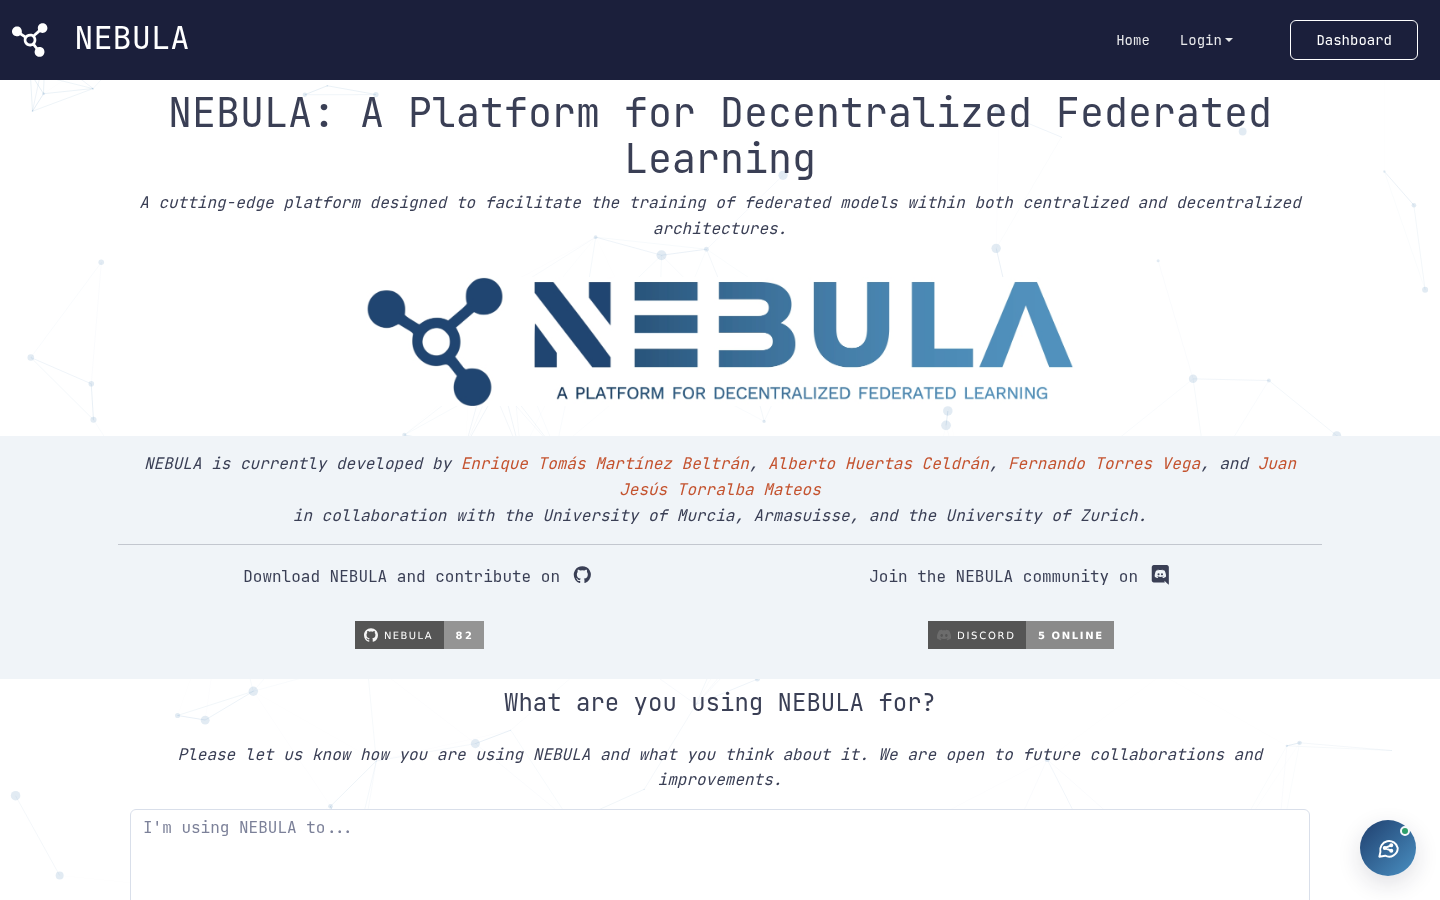
\includegraphics[width=0.95\columnwidth,height=5.5cm,keepaspectratio]{imagenes/04_web_register_result.png}
    \caption{\footnotesize Home page after the web account was created (redirect from \texttt{POST /platform/register}).}
    \label{fig:web-register-result}
\end{figure}

% ------------------------------------------------------------
\subsection{Part 8: JWT Authentication}

Tokens are created in \texttt{security/jwt.py} with \texttt{python-jose} and the HS256 algorithm. The secret is read from the \texttt{JWT\_SECRET} environment variable, and the application refuses to start if it is missing. Every token carries the claims \texttt{sub} (user id), \texttt{type} (\texttt{access} or \texttt{refresh}), \texttt{jti} (unique identifier), \texttt{iat} and \texttt{exp}.

\begin{itemize}
    \item The \textbf{access token} lasts 15 minutes (\texttt{ACCESS\_TOKEN\_MINUTES}) and is sent in the header \texttt{Authorization: Bearer <access-token>}.
    \item The \textbf{refresh token} lasts 7 days (\texttt{REFRESH\_TOKEN\_DAYS}), or 30 days with \textit{Remember Me}, and is only used to obtain new tokens.
\end{itemize}

The function \texttt{decode\_token} verifies the signature, the expiration and the \texttt{type} claim, so a refresh token cannot be used as an access token, and vice versa. Both cases are covered by automated tests. The dependency \texttt{get\_current\_user} additionally checks that the user still exists and is active, and answers 401 with \texttt{WWW-Authenticate: Bearer} otherwise.

% ------------------------------------------------------------
\subsection{Part 9: Login}

\texttt{POST /auth/login} receives JSON with \texttt{email}, \texttt{password} and \texttt{remember\_me} and returns:

\begin{lstlisting}[basicstyle=\ttfamily\footnotesize]
{"access_token": "eyJ...",
 "refresh_token": "eyJ...",
 "token_type": "bearer",
 "expires_in": 900}
\end{lstlisting}

An incorrect password, an unknown email and a social-only account all produce the same response, \texttt{401 Invalid email or password}, and the same computation cost (a decoy hash is verified when the account does not exist), so the endpoint does not reveal whether an account exists. A disabled account receives 403. On success, the refresh token is registered in the database and \texttt{last\_login} is updated. The Postman evidence for this endpoint is shown in Figs.~\ref{fig:postman-login-body} and \ref{fig:postman-login-respuesta}.

NEBULA's web login (\texttt{POST /platform/login}, session cookie) is unchanged and independent. It was tested in the browser with the QA account: the endpoint answers \texttt{\{"message": "Login successful"\}} and the session is kept, so the navbar switches from \textit{Login} to \textit{Account} (Fig.~\ref{fig:web-logged-in}).

\begin{figure}[H]
    \centering
    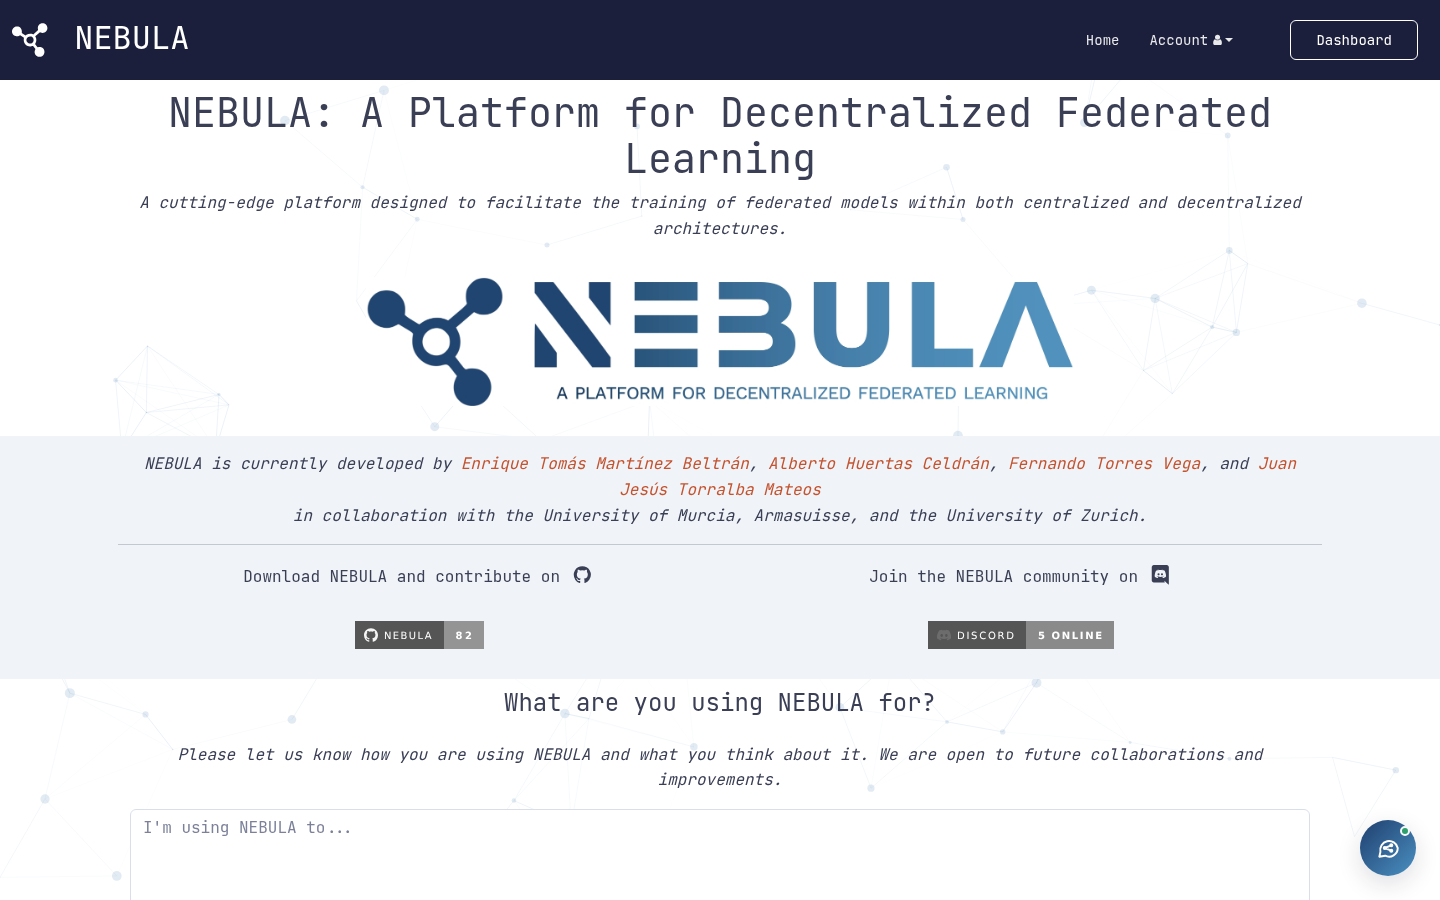
\includegraphics[width=0.95\columnwidth,height=5.5cm,keepaspectratio]{imagenes/05_web_logged_in.png}
    \caption{\footnotesize Web interface after login: the navbar shows \textit{Account} instead of \textit{Login}.}
    \label{fig:web-logged-in}
\end{figure}

% ------------------------------------------------------------
\subsection{Part 10: Remember Me}

The \texttt{remember\_me} field of the login request changes only the lifetime of the refresh token: 7 days when \texttt{false} and 30 days when \texttt{true}. The access token always lasts 15 minutes (900~s). The choice is stored in the \texttt{remember\_me} column of the session, and token rotation keeps it, so a user who selected \textit{Remember Me} keeps the extended lifetime after each refresh. A test decodes both refresh tokens and verifies 7 and 30 days, and that the access token of the \textit{Remember Me} login still lasts 900~s.

% ------------------------------------------------------------
\subsection{Part 11: Refresh Tokens}

\texttt{POST /auth/refresh} receives \texttt{\{"refresh\_token": "eyJ..."\}}. The API verifies that the signature is valid, the token has not expired, its type is \texttt{refresh}, its hash exists in the database, it has not been revoked, and the user still exists and is active. Any failure produces the same response, \texttt{401 Invalid refresh token}.

The endpoint implements the \textbf{refresh-token rotation} of the workshop: the used token is revoked and a new access and refresh pair is issued. In addition, if a token that was already revoked (rotated or closed by logout) is presented again, the API assumes it may have been stolen and revokes \textbf{all} active sessions of that user. Tests cover rotation, rejection of the old token, reuse detection, a malformed token, and a correctly signed token that is not in the database.

% ------------------------------------------------------------
\subsection{Part 12: Logout}

Logout revokes the session in the database by setting \texttt{revoked\_at} in the \texttt{refresh\_tokens} table (Table~\ref{tab:api-refresh}). Only the SHA-256 hash of each refresh token is stored.

\begin{itemize}
    \item \texttt{POST /auth/logout} receives the refresh token and revokes it. It is idempotent: it always answers 204 No Content.
    \item \texttt{POST /auth/logout-all} (extra endpoint, requires a Bearer access token) revokes all active sessions of the user.
\end{itemize}

After logout, using that refresh token returns 401. An access token already issued remains valid until it expires (at most 15 minutes), because access tokens are stateless; the optional denylist with \texttt{jti} was not implemented.

NEBULA's web logout (\texttt{GET /platform/logout}) is unchanged. It removes only the \texttt{user} key from the session; replacing \texttt{session.pop("user")} with \texttt{session.clear()} is a pending fix for the web application.

% ------------------------------------------------------------
\subsection{Part 13: Current Authenticated User}

\texttt{GET /users/me} requires a Bearer access token and returns the authenticated user: \texttt{id}, \texttt{username}, \texttt{full\_name}, \texttt{email}, \texttt{role}, \texttt{auth\_provider} and \texttt{created\_at}. It never returns the password hash. Without a token, with an invalid or expired token, or with a refresh token, it answers 401.

% ------------------------------------------------------------
\subsection{Part 14: Social registration and login}

Google is integrated through OAuth 2.0 / OpenID Connect with Authlib, in \texttt{routers/social.py}. The flow runs on the server:

\begin{enumerate}
    \item \texttt{GET /auth/google/login} redirects the browser to Google. The \texttt{state} parameter is kept in a signed session cookie (\texttt{SessionMiddleware}).
    \item After authentication and consent, Google redirects to \texttt{GET /auth/google/callback}.
    \item The server exchanges the code and receives the user information from Google. It requires a verified email.
    \item It finds the user by (\texttt{auth\_provider}, \texttt{provider\_user\_id}) or creates one with the email as username, \texttt{auth\_provider = google}, the Google identifier in \texttt{provider\_user\_id} and \texttt{password\_hash = NULL}.
    \item It returns the application's own access and refresh tokens, the same as \texttt{/auth/login}.
\end{enumerate}

The Google password is never received or stored, and a social account cannot log in with a password. If the email already exists as a local account, the API answers \texttt{409 Conflict} instead of linking the accounts automatically, which avoids account takeover. If the Google credentials are not configured (\texttt{GOOGLE\_CLIENT\_ID}, \texttt{GOOGLE\_CLIENT\_SECRET}), \texttt{/auth/google/login} answers 503 and the rest of the API works normally. The \texttt{/auth/google/login} endpoint must be opened in a browser tab, not with \textit{Try it out}, because it redirects, and \texttt{127.0.0.1} must be used consistently (not mixed with \texttt{localhost}) so the \texttt{state} cookie is kept.

The server completes the OAuth exchange itself, so it does not trust an identity sent by the browser. The automated tests verify user creation, reuse of an existing social user, the 409 rule, and that a social account cannot use \texttt{/auth/login}. The NEBULA web interface keeps its existing Google sign-in through Firebase (\texttt{signInWithPopup} and \texttt{POST /platform/firebase\_auth}).

No real Google credentials were configured in this project (\texttt{GOOGLE\_CLIENT\_ID} and \texttt{GOOGLE\_CLIENT\_SECRET} are empty in \texttt{.env}), so \texttt{GET /auth/google/login} correctly answers 503, as shown in Fig.~\ref{fig:google-not-configured}. This behavior is covered by the automated test \texttt{test\_social\_login\_not\_configured\_returns\_503}, and the same 503 appears in the Postman Runner (Fig.~\ref{fig:postman-run-completo}) and in the browser end-to-end run (Fig.~\ref{fig:browser-qa-flow}). The social user logic (creation, reuse, 409 on email collision, \texttt{password\_hash = NULL}, rejection on \texttt{/auth/login}) is verified by \texttt{test\_social\_user\_creation\_and\_linking\_rules} and \texttt{test\_social\_only\_account\_cannot\_login\_with\_password}. The complete browser round-trip with real Google credentials (consent screen $\rightarrow$ callback $\rightarrow$ \texttt{GET /users/me} with \texttt{"auth\_provider": "google"}) remains pending and requires valid credentials plus the redirect URI. On the web side, the \textit{Sign in with Google} button (Firebase \texttt{signInWithPopup} $\rightarrow$ \texttt{POST /platform/firebase\_auth}) is visible in the login dropdown and on the sign-up page (Fig.~\ref{fig:web-register-form}); completing it also requires authorizing the domain in the Firebase console, so it was not executed in this headless test.

\begin{figure}[H]
    \centering
    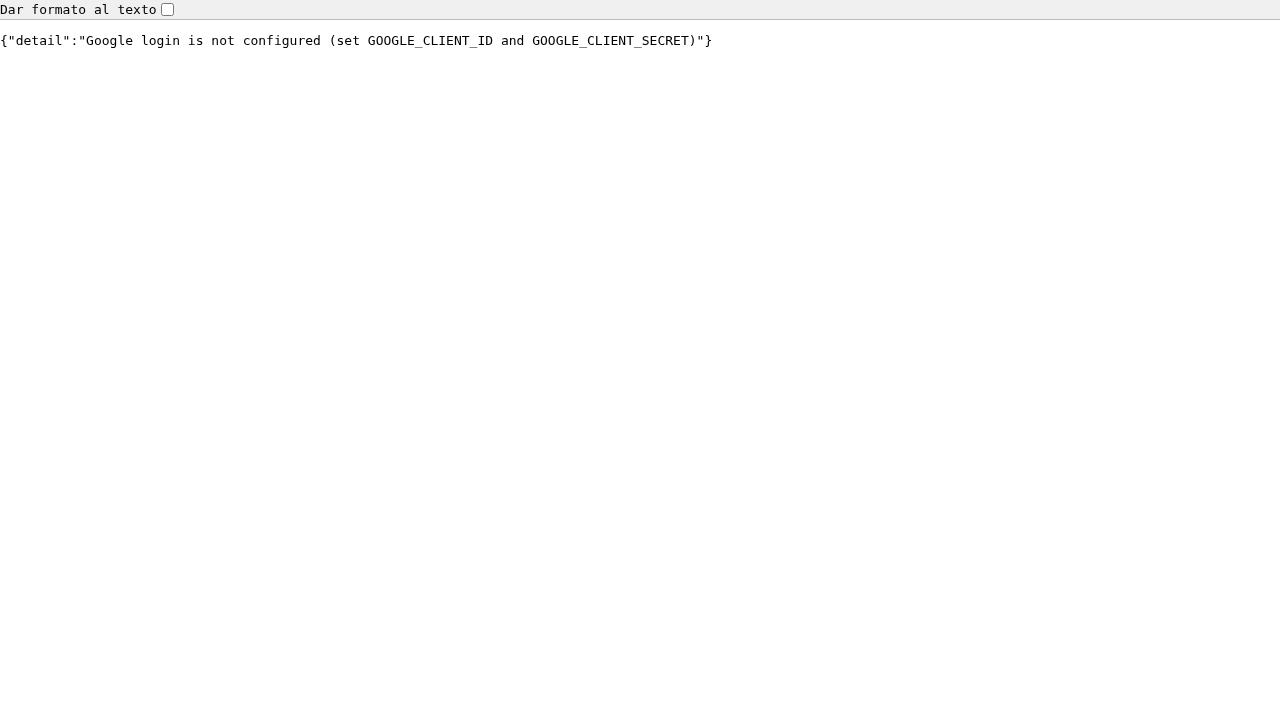
\includegraphics[width=0.95\columnwidth,height=2.8cm,keepaspectratio]{imagenes/06_api_google_503.png}
    \caption{\footnotesize \texttt{GET /auth/google/login} without credentials returns 503 with a JSON detail.}
    \label{fig:google-not-configured}
\end{figure}


% ------------------------------------------------------------
\subsection{Part 15: Public Endpoints}

Four JSON endpoints that do not require authentication were added under the \textit{Public} tag:

\begin{itemize}
    \item \texttt{GET /public/info}: \texttt{\{"api": "NEBULA API", "version": "1.0", "authentication\_required": false\}}.
    \item \texttt{GET /public/datasets}: supported datasets, each with its models.
    \item \texttt{GET /public/aggregators}: \texttt{FedAvg}, \texttt{Krum}, \texttt{Median}, \texttt{TrimmedMean}.
    \item \texttt{GET /public/topologies}: federation types (\texttt{DFL}, \texttt{SDFL}, \texttt{CFL}) and topologies (\texttt{Fully}, \texttt{Ring}, \texttt{Star}, \texttt{Random}).
\end{itemize}

They are useful because their values are exactly those accepted when an experiment is created. The standalone application also exposes \texttt{GET /}, which returns \texttt{\{"message": "NEBULA API", "version": "1.0.0"\}}. Figure~\ref{fig:public-info} shows the real response of \texttt{GET /public/info} obtained in the browser.

\begin{figure}[H]
    \centering
    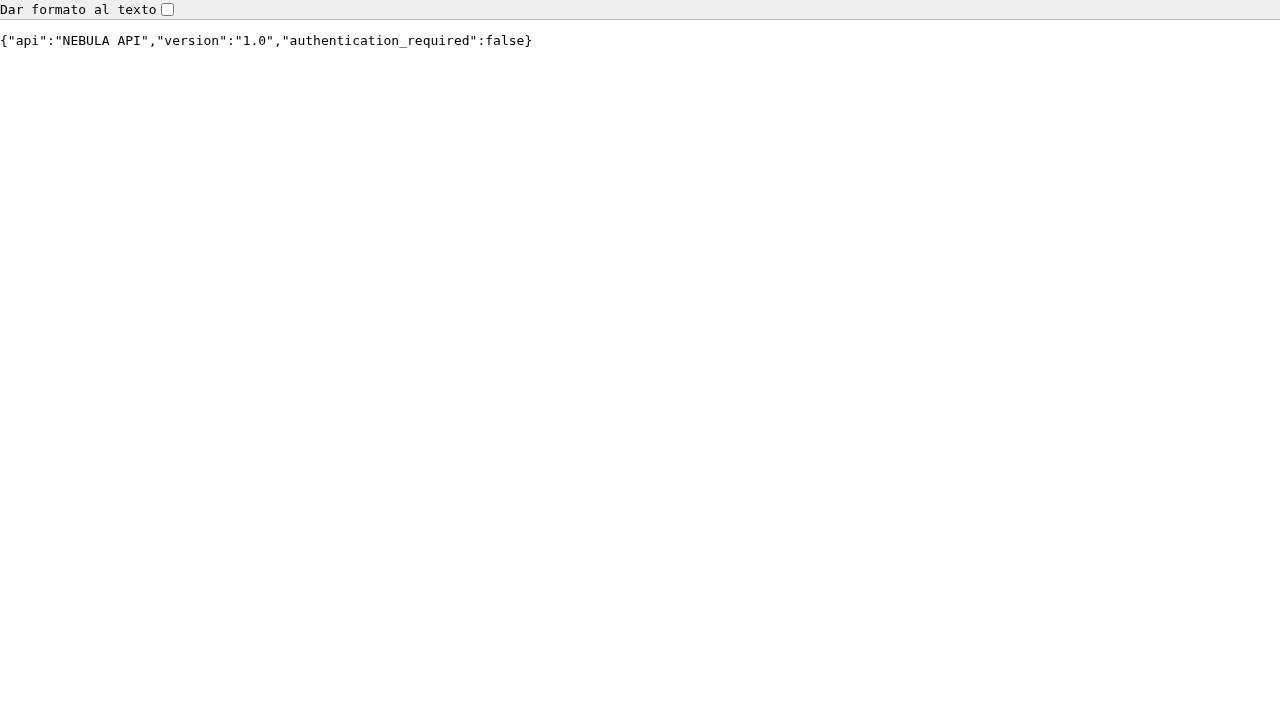
\includegraphics[width=0.95\columnwidth,height=2.8cm,keepaspectratio]{imagenes/07_api_public_info.png}
    \caption{\footnotesize \texttt{GET /public/info} returns the API name, version and no-authentication flag.}
    \label{fig:public-info}
\end{figure}

The data comes from \texttt{catalog.py}, which is based on the datasets, models and aggregators of NEBULA but does not match them exactly. Some CIFAR10 model names differ from those used by the platform (\texttt{ResNet}, \texttt{FasterMobileNet} and \texttt{SimpleMobileNet} instead of \texttt{ResNet9}, \texttt{fastermobilenet} and \texttt{simplemobilenet}). \texttt{Sentiment140} is listed although NEBULA has no dataset loader for it. The tabular datasets Covtype, AdultCensus and BreastCancer, which NEBULA supports, are not included.

% ------------------------------------------------------------
\subsection{Part 16: Group's Entity}

The application entity of the REST API is \texttt{Experiment}: the configuration of a federated-learning experiment that belongs to a user (Table~\ref{tab:api-experiments}). It matches what NEBULA already handles as a scenario and can later feed \texttt{/scenarios/run}. The relationship is one user to many experiments, established by \texttt{user\_id}. The owner is always taken from the JWT; a \texttt{user\_id} sent in the body is ignored.

The schema \texttt{ExperimentCreate} validates ranges (for example \texttt{n\_nodes} between 2 and 50) and that the \texttt{model} is valid for the chosen \texttt{dataset} (for example \texttt{MNIST} accepts \texttt{MLP} and \texttt{CNN}, but not \texttt{ResNet}). Complete CRUD is implemented (Table~\ref{tab:crud}), with \texttt{PATCH} added to the five operations of the workshop. \texttt{PATCH} merges the sent fields and validates the whole result, so changing the dataset without changing the model is rejected with 422.

\begin{table}[H]
\centering
\scriptsize
\begin{tabularx}{\columnwidth}{l l X}
\hline
\textbf{Method} & \textbf{Endpoint} & \textbf{Description and responses} \\
\hline
POST   & \texttt{/experiments}      & Create. 201 / 401 / 422 \\
GET    & \texttt{/experiments}      & List only the user's experiments, newest first; filters \texttt{status}, \texttt{skip}, \texttt{limit}. 200 / 401 \\
GET    & \texttt{/experiments/\{id\}} & Read. 200 / 401 / 403 / 404 \\
PUT    & \texttt{/experiments/\{id\}} & Replace (all fields). 200 / 401 / 403 / 404 / 422 \\
PATCH  & \texttt{/experiments/\{id\}} & Partial update. 200 / 401 / 403 / 404 / 422 \\
DELETE & \texttt{/experiments/\{id\}} & Delete. 204 / 401 / 403 / 404 \\
\hline
\end{tabularx}
\caption{CRUD of the \texttt{Experiment} entity (all routes require a Bearer access token).}
\label{tab:crud}
\end{table}

\paragraph{SMAC functionality.} The project's main contribution, SMAC, is an orchestration assistant for federated-learning scenarios in the web application (port 6060). It works with \textit{SMAC actions} (commands proposed by the chatbot and confirmed by a human, with \texttt{id}, \texttt{kind}, \texttt{params}, \texttt{description}, \texttt{scenario}, \texttt{username} and \texttt{expires\_at}; kinds \texttt{pause\_node}, \texttt{resume\_node}, \texttt{select\_aggregator}, \texttt{propose\_disconnect} and \texttt{stop\_scenario}) and with \textit{scenario metrics} read from TensorBoard logs. Actions are kept in memory and expire after 600 seconds, so they do not form a CRUD; for this reason the CRUD of the workshop is implemented on \texttt{Experiment}. The assistant uses the Groq API (model \texttt{openai/gpt-oss-120b}), configured with \texttt{GROQ\_API\_KEY}, and four agents on each node (StragglerPredictor, AggregationSelector, ResourceBroker, GroqReasoning) suggest commands to NEBULA's situational-awareness module. Its endpoints (Table~\ref{tab:smac-endpoints}) are protected by the web session.

\begin{table}[H]
\centering
\scriptsize
\begin{tabularx}{\columnwidth}{l >{\raggedright\arraybackslash}X}
\hline
\textbf{Method} & \textbf{Endpoint and description} \\
\hline
POST & \texttt{/platform/smac/chat/}: ask the assistant; returns a reply and proposed actions \\
POST & \texttt{/platform/smac/propose}: create a pending action \\
POST & \texttt{/platform/smac/chat/confirm}: confirm or reject a pending action \\
POST & \texttt{/platform/api/smac/actions/execute}: execute an action with a confirmation token \\
POST & \texttt{/platform/smac/analyze}: generate an LLM situation report \\
GET & \texttt{/platform/smac/state}: current scenario state (nodes, edges, round, stragglers) \\
GET & \texttt{/platform/api/smac/events}: live events (server-sent events) \\
GET & \texttt{/platform/api/scenarios}: scenarios of the current user \\
GET & \texttt{/platform/api/scenarios/\{id\}/summary}: scenario summary \\
GET & \texttt{/platform/api/scenarios/\{id\}/metrics}: metric series with filters \\
GET & \texttt{/platform/api/scenarios/\{id\}/events}: scenario events \\
\hline
\end{tabularx}
\caption{Endpoints of the SMAC functionality (web application, session-protected).}
\label{tab:smac-endpoints}
\end{table}

% ------------------------------------------------------------
\subsection{Part 17: JWT Authorization}

Authentication answers \textit{who is this user?} and authorization answers \textit{may this user perform this operation?}. In the API both questions are addressed:

\begin{itemize}
    \item \textbf{Authentication:} every \texttt{/experiments} route and \texttt{/users/me} depend on \texttt{get\_current\_user}, which validates the Bearer access token and the state of the user. Without a valid token the answer is 401.
    \item \textbf{Authorization:} the function \texttt{get\_owned\_experiment} is used by read, replace, patch and delete. It answers 404 if the experiment does not exist and 403 if it belongs to another user. The list endpoint filters by the authenticated user, so other users' experiments never appear.
\end{itemize}

A user therefore cannot read, modify or delete another user's experiment by changing the id in the URL, which is verified by a test for GET, PUT, PATCH and DELETE. If it is preferred not to reveal that a resource exists, the 403 can be replaced by 404 in that single function.

In the web application, the SMAC and metrics endpoints are protected by the session. They return 401 without a session, \texttt{admin} can confirm every action, \texttt{user} can confirm every action except \texttt{stop\_scenario}, and other roles have read-only access. The scenario endpoints (\texttt{/platform/api/scenarios/\{id\}/...}) verify that the user may access the scenario. The chat, state, analyze, propose and events endpoints do not yet check scenario ownership, so this verification is pending.

% ------------------------------------------------------------
\subsection{Part 18: JSON responses}

All the endpoints of the REST API receive and return JSON, including errors, which use the form \texttt{\{"detail": ...\}}. Creation returns the complete entity:

\begin{lstlisting}[basicstyle=\ttfamily\footnotesize]
POST /experiments  ->  201 Created
{"id": 1, "name": "MNIST ring FedAvg",
 "federation": "DFL", "topology": "Ring",
 "dataset": "MNIST", "model": "MLP",
 "agg_algorithm": "FedAvg", "n_nodes": 4,
 "rounds": 3, "epochs": 1, "status": "draft",
 "user_id": 5, "created_at": "...",
 "updated_at": "..."}
\end{lstlisting}

The status codes used are 200 (success), 201 (created), 204 (no content: logout and delete), 302 (redirect to Google), 401 (missing, invalid, expired or revoked token; wrong credentials), 403 (inactive account or resource of another user), 404 (resource not found), 409 (duplicate account or email already used by another sign-in method), 422 (validation error) and 503 (Google login not configured). No endpoint of the API returns HTML except the Swagger documentation pages.

In the web application, NEBULA's global exception handler (\texttt{custom\_http\_exception\_handler} in \texttt{frontend/app.py}) renders 401, 403 and 404 errors as HTML pages, and the web registration returns redirects. This applies to the web interface (port 6060), not to the REST API.

% ------------------------------------------------------------
\subsection{Part 19: Improve OpenAPI documentation}

The documentation of the REST API follows the workshop's guidelines (Part~4): tags, summaries, descriptions, Pydantic request and response models with examples, documented status codes, and an \texttt{HTTPBearer} security scheme. Authentication is declared with \texttt{HTTPBearer(auto\_error=False)}, which has two effects: Swagger UI shows the \textit{Authorize} button, and a missing header produces 401 instead of the default 403. A test verifies that the generated specification contains the \texttt{HTTPBearer} scheme, the tags and the experiment routes.

% ------------------------------------------------------------
\subsection{Part 20: Test authentication with Swagger UI}

Swagger UI is available at \texttt{http://127.0.0.1:8000/docs}. The sequence is: test \texttt{GET /public/info}; register with \texttt{POST /auth/register}; log in with \texttt{POST /auth/login} and copy the \texttt{access\_token}; press \textit{Authorize} and paste only the token (without the word \textit{Bearer}); call \texttt{GET /users/me}; and test the \textit{Experiments} CRUD. Because the login receives JSON, the OAuth2 password form of Swagger UI is not used; HTTP Bearer authorization is used instead. Figure~\ref{fig:swagger-docs} shows the documented API in Swagger UI with the \textit{Authorize} button and the five tag groups.

\begin{figure}[H]
    \centering
    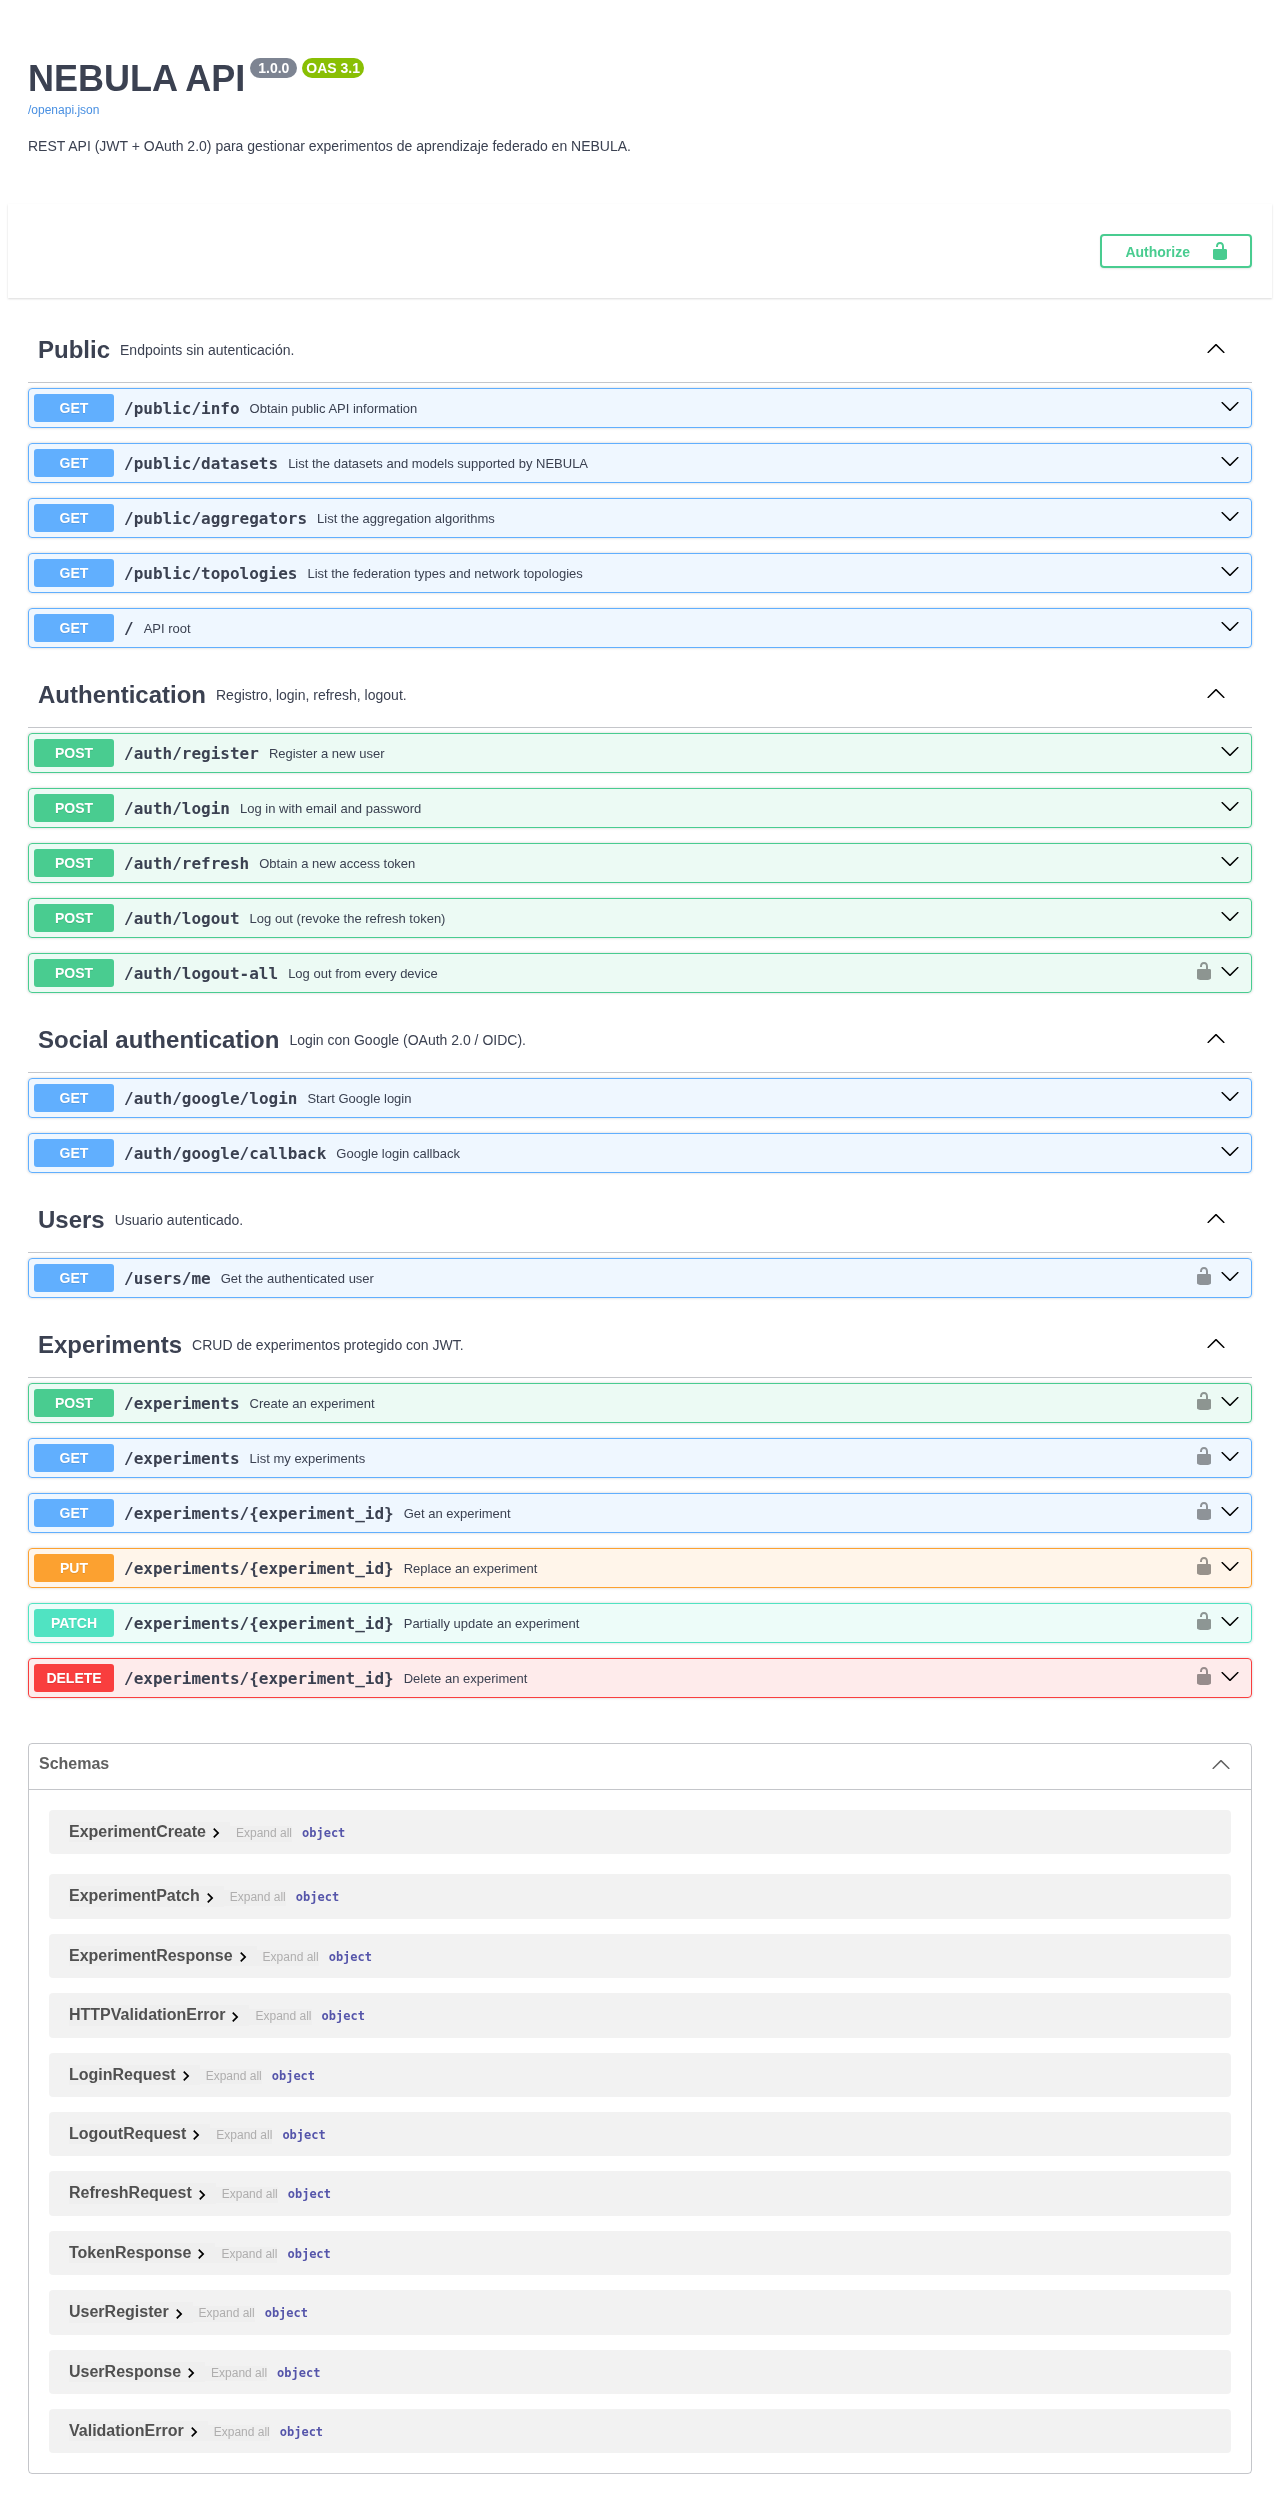
\includegraphics[width=0.95\columnwidth,height=6.5cm,keepaspectratio]{imagenes/08_swagger_docs.png}
    \caption{\footnotesize Swagger UI of the standalone API with the Public, Authentication, Social, Users and Experiments groups.}
    \label{fig:swagger-docs}
\end{figure}

The invalid cases (\texttt{GET /users/me} without token, an invented token such as \texttt{abc}, and an expired token, all answered with 401) are covered by the automated tests \texttt{test\_users\_me} and \texttt{test\_invalid\_and\_expired\_tokens\_rejected}, which generate an expired token with the same secret and an \texttt{exp} in the past. The same session flow was additionally verified end-to-end in the browser: Fig.~\ref{fig:browser-qa-flow} shows register (201), login (200), \texttt{/users/me} (200), refresh (200), logout (204), refresh-after-logout rejected with 401, and Google login answered with 503 because no credentials are configured.

\begin{figure}[H]
    \centering
    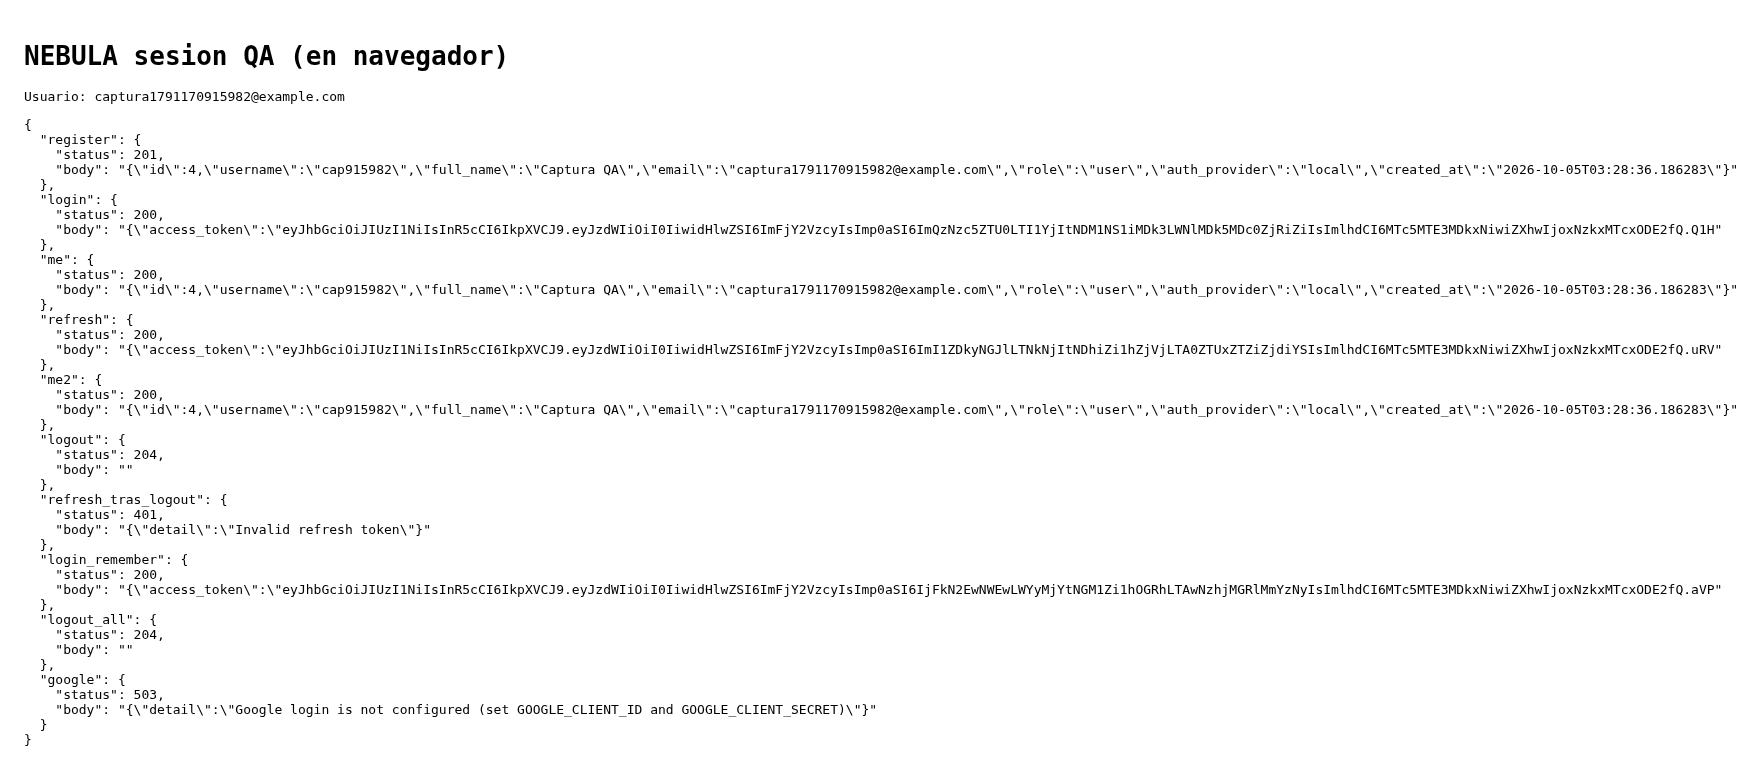
\includegraphics[width=0.95\columnwidth,height=5.5cm,keepaspectratio]{imagenes/09_browser_qa_flow.png}
    \caption{\footnotesize Browser end-to-end run: register, login, \texttt{/users/me}, refresh, logout, rejected reuse (401) and Google 503.}
    \label{fig:browser-qa-flow}
\end{figure}

% ------------------------------------------------------------
\subsection{Part 21: Test with Postman}

The collection \textit{NEBULA-Sesion} uses the environment variables \texttt{base\_url = http://127.0.0.1:8000}, \texttt{access\_token}, \texttt{refresh\_token} and \texttt{experiment\_id}. Protected requests use \textit{Bearer Token} authorization with \texttt{\{\{access\_token\}\}}, and the request bodies are raw JSON. Test scripts store the tokens automatically after \texttt{login} and \texttt{refresh}, and the experiment id after creation:

\begin{lstlisting}[language=Java, basicstyle=\ttfamily\footnotesize]
const j = pm.response.json();
pm.environment.set("access_token",
                   j.access_token);
pm.environment.set("refresh_token",
                   j.refresh_token);
\end{lstlisting}

The recommended sequence is: public endpoints; register; login; \texttt{/users/me}; create, list, read, replace and patch an experiment; refresh (the old refresh token must then return 401); logout (the refresh token must then return 401); and logout-all. The negative cases are \texttt{/users/me} and \texttt{/experiments} without a token (401), another user's experiment (403), invalid registration (409, 422) and a wrong password (401). For \textit{Remember Me}, the refresh token can be decoded at jwt.io and the difference between \texttt{exp} and \texttt{iat} should be about 7 or 30 days, with the access token always at 900~s. An importable collection with the main requests is included in the project documentation (\texttt{NEBULA-Sesion.postman\_collection.json}). Figure~\ref{fig:postman-collection} shows the imported collection with its documented session flow, and the execution evidence follows in Figs.~\ref{fig:postman-register-body}--\ref{fig:postman-run-completo}.

\begin{figure}[H]
    \centering
    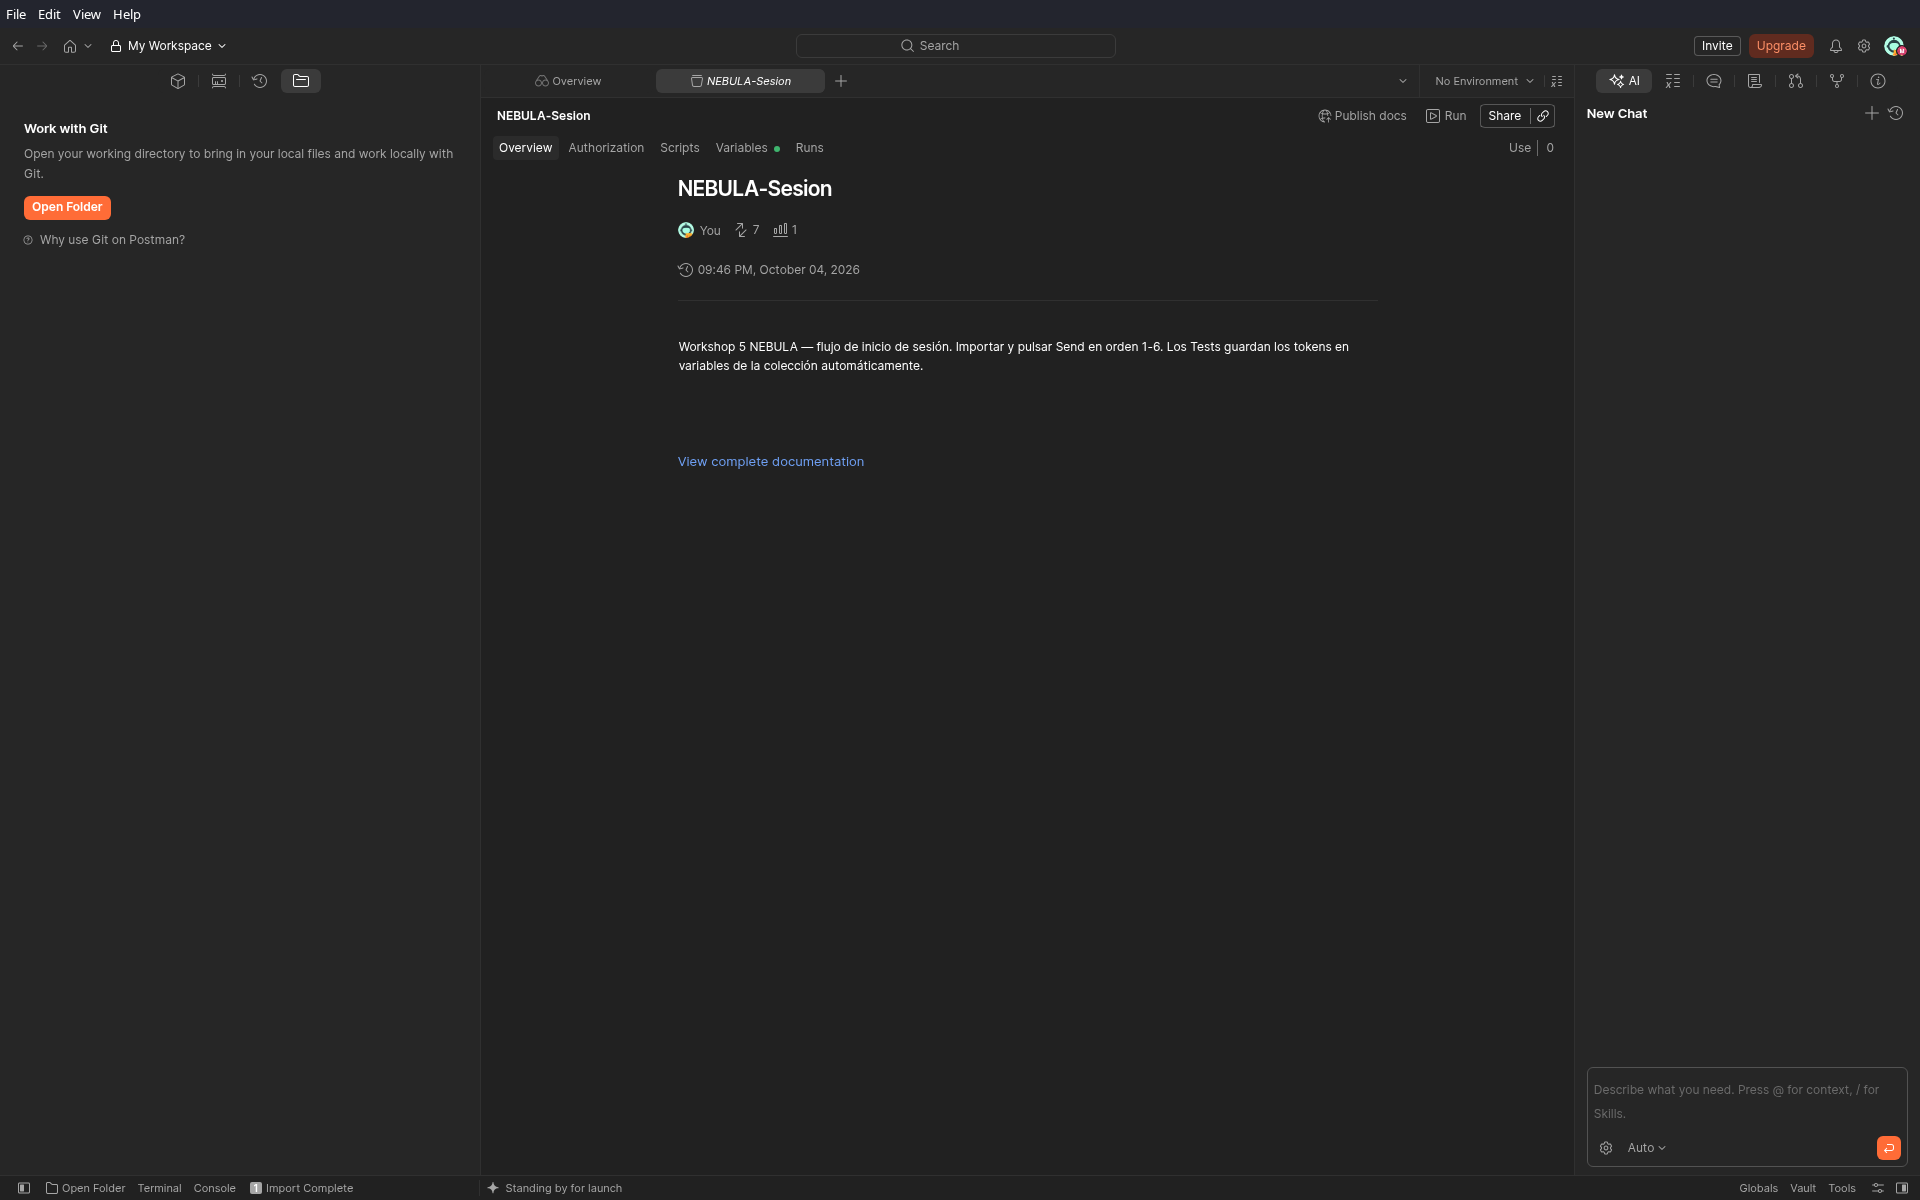
\includegraphics[width=0.95\columnwidth,height=5.5cm,keepaspectratio]{imagenes/10_postman_coleccion.png}
    \caption{\footnotesize Postman collection \textit{NEBULA-Sesion} with the documented session flow.}
    \label{fig:postman-collection}
\end{figure}

Figure~\ref{fig:postman-register-body} shows the raw JSON body sent to \texttt{POST /auth/register} (\texttt{username}, \texttt{full\_name}, \texttt{email}, \texttt{password}).

\begin{figure}[H]
    \centering
    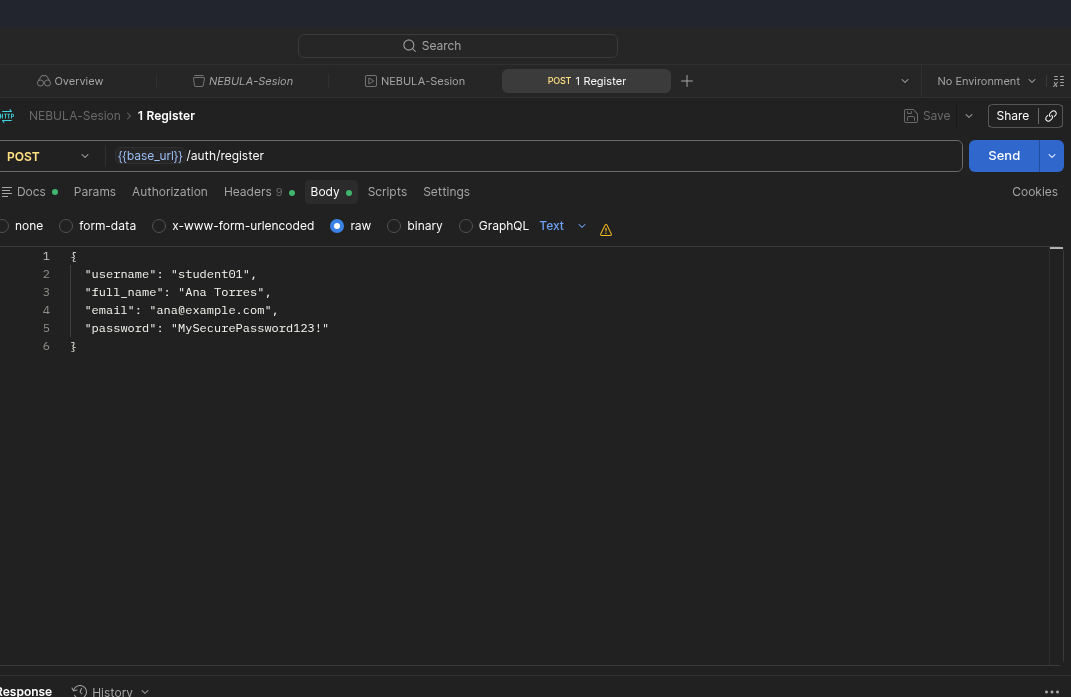
\includegraphics[width=0.95\columnwidth,height=5.5cm,keepaspectratio]{imagenes/11_postman_register_body.png}
    \caption{\footnotesize Postman: JSON body sent to \texttt{POST /auth/register}.}
    \label{fig:postman-register-body}
\end{figure}

Figure~\ref{fig:postman-register-respuesta} shows its response: \texttt{201 Created} with the created user (\texttt{id}, \texttt{username}, \texttt{full\_name}, \texttt{email}, \texttt{role}, \texttt{auth\_provider}, \texttt{created\_at}) and no password hash.

\begin{figure}[H]
    \centering
    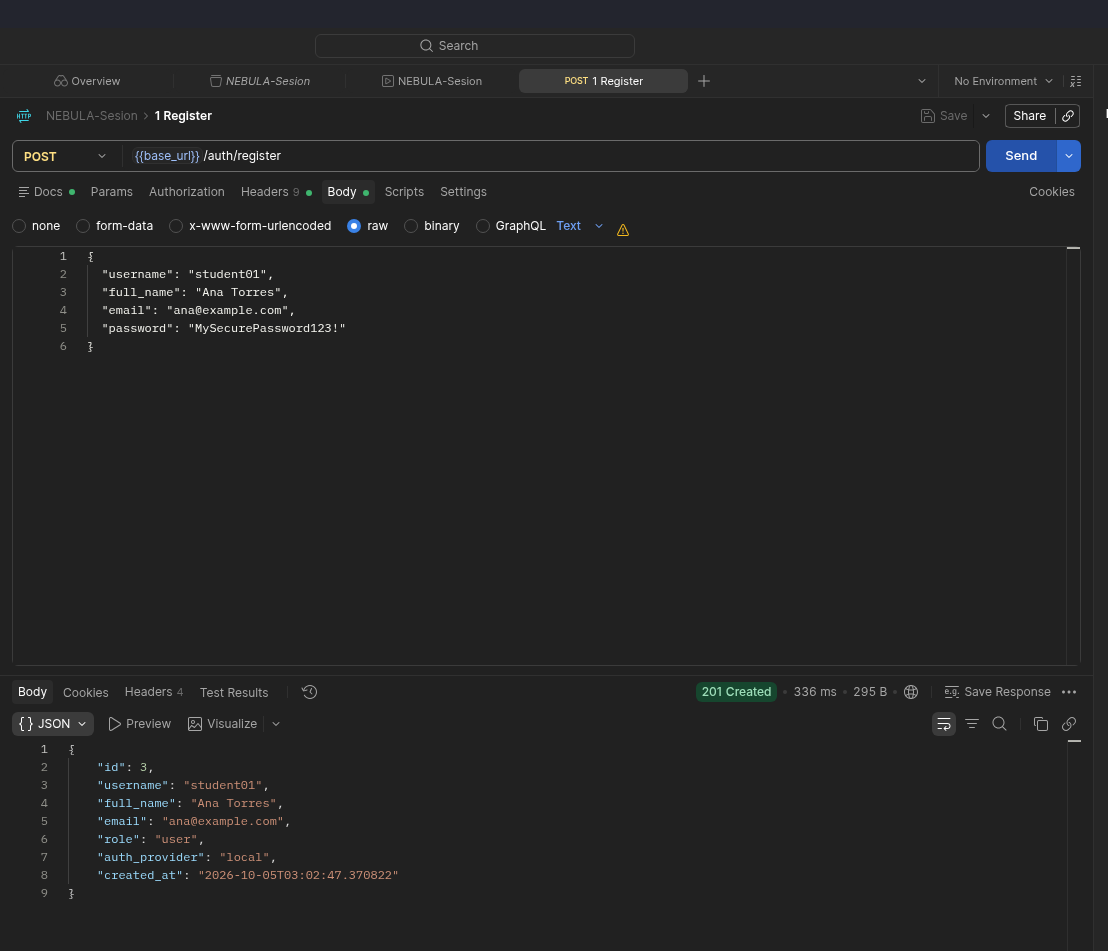
\includegraphics[width=0.95\columnwidth,height=5.5cm,keepaspectratio]{imagenes/12_postman_register_201.png}
    \caption{\footnotesize Postman: \texttt{201 Created} on register, returning the user without password hash.}
    \label{fig:postman-register-respuesta}
\end{figure}

Figure~\ref{fig:postman-login-body} shows the raw JSON body sent to \texttt{POST /auth/login} (\texttt{email}, \texttt{password}, \texttt{remember\_me} in false).

\begin{figure}[H]
    \centering
    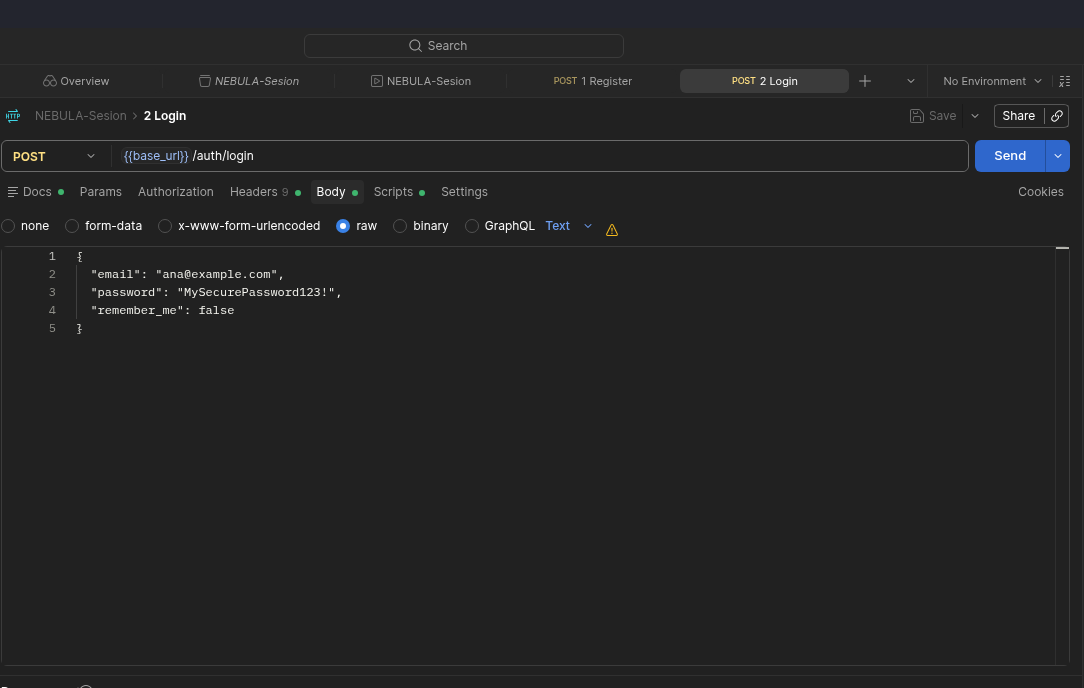
\includegraphics[width=0.95\columnwidth,height=5.5cm,keepaspectratio]{imagenes/13_postman_login_body.png}
    \caption{\footnotesize Postman: JSON body sent to \texttt{POST /auth/login} with \texttt{remember\_me} in false.}
    \label{fig:postman-login-body}
\end{figure}

Figure~\ref{fig:postman-login-respuesta} shows its response: \texttt{200 OK} with \texttt{access\_token}, \texttt{refresh\_token}, \texttt{token\_type} bearer and \texttt{expires\_in} 900.

\begin{figure}[H]
    \centering
    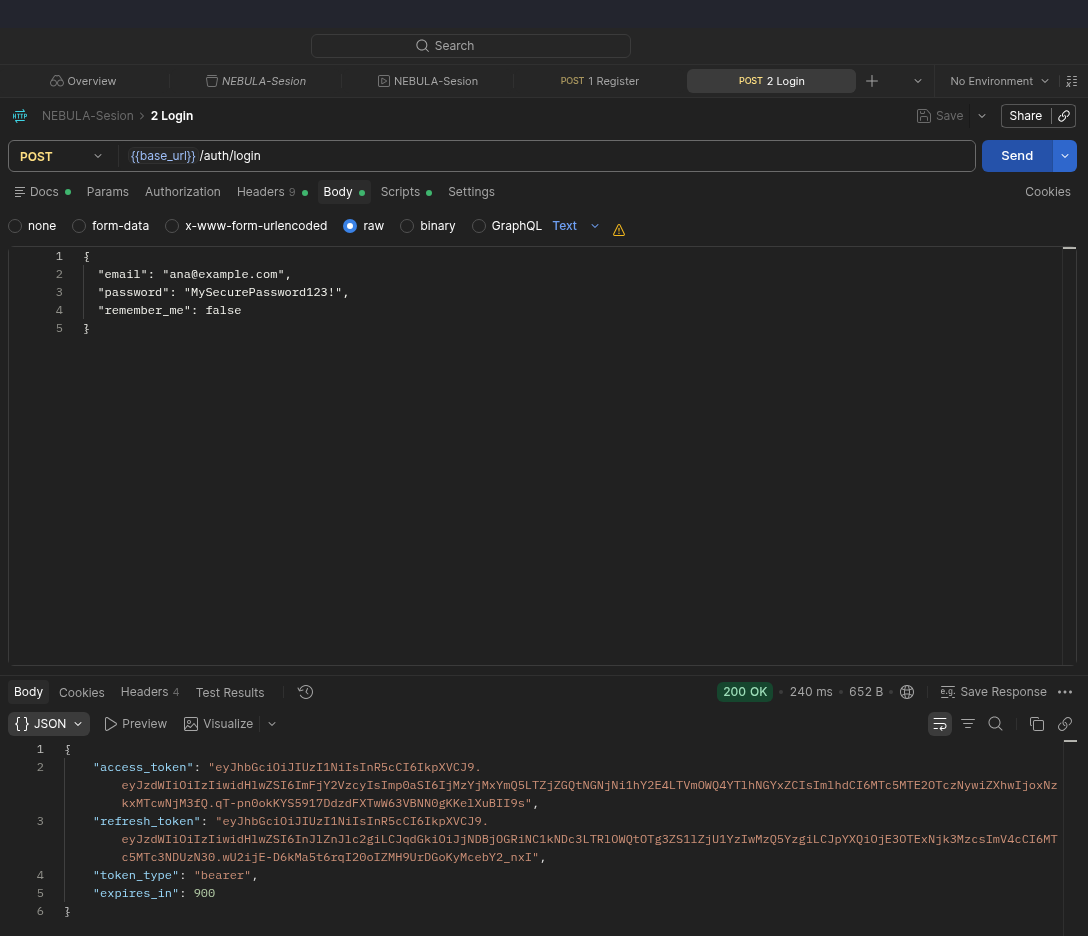
\includegraphics[width=0.95\columnwidth,height=5.5cm,keepaspectratio]{imagenes/14_postman_login_200.png}
    \caption{\footnotesize Postman: \texttt{200 OK} on login with access token, refresh token and \texttt{expires\_in} 900.}
    \label{fig:postman-login-respuesta}
\end{figure}

Figure~\ref{fig:postman-run-201} shows the first collection run in the Postman Runner: \texttt{POST /auth/register} returns 201, \texttt{POST /auth/login}, \texttt{GET /users/me} and \texttt{POST /auth/refresh} return 200, and \texttt{POST /auth/logout} returns 204.

\begin{figure}[H]
    \centering
    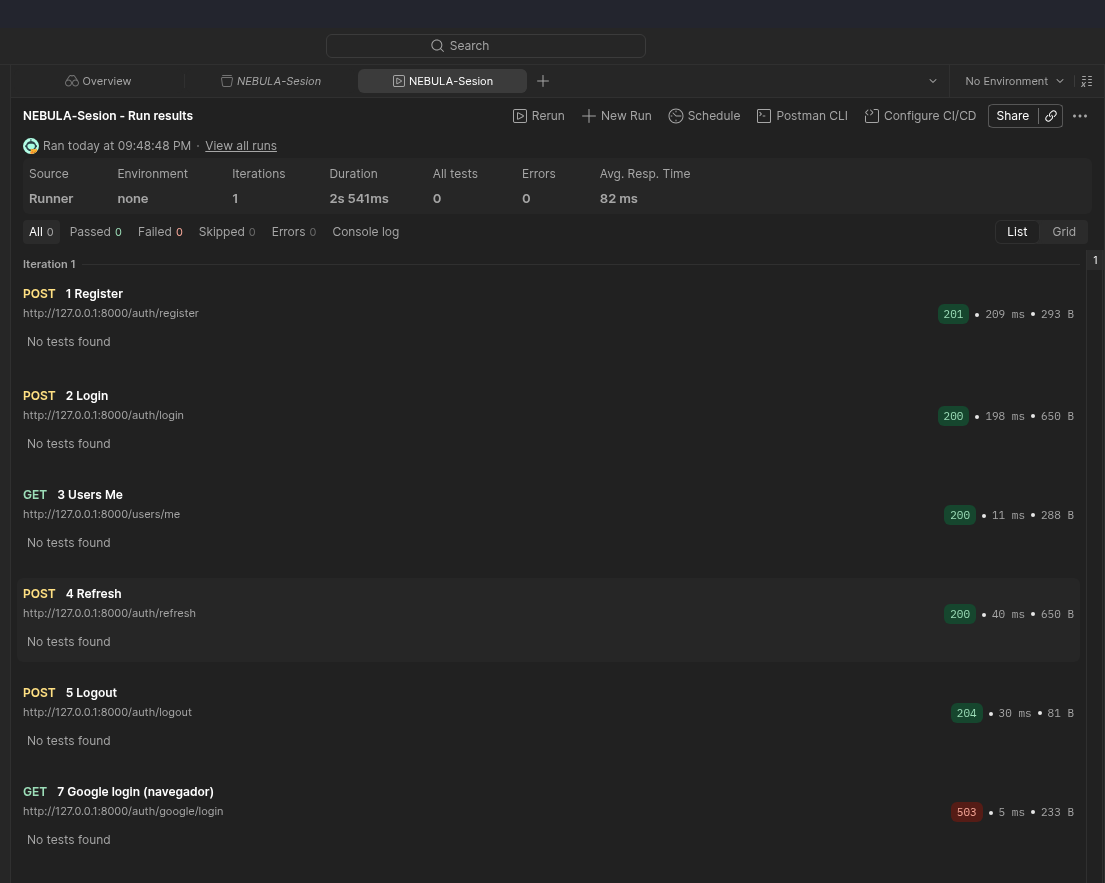
\includegraphics[width=0.95\columnwidth,height=5.5cm,keepaspectratio]{imagenes/15_postman_run_201.png}
    \caption{\footnotesize Postman Runner: first run with 201 on register and 200/204 on login, \texttt{/users/me}, refresh and logout.}
    \label{fig:postman-run-201}
\end{figure}

Figure~\ref{fig:postman-run-completo} shows the complete run once the user already exists: the repeated register is correctly rejected with 409, while login, \texttt{/users/me}, refresh, logout and logout-all succeed (200/204). The Google login request returns 503 because no real Google credentials are configured.

\begin{figure}[H]
    \centering
    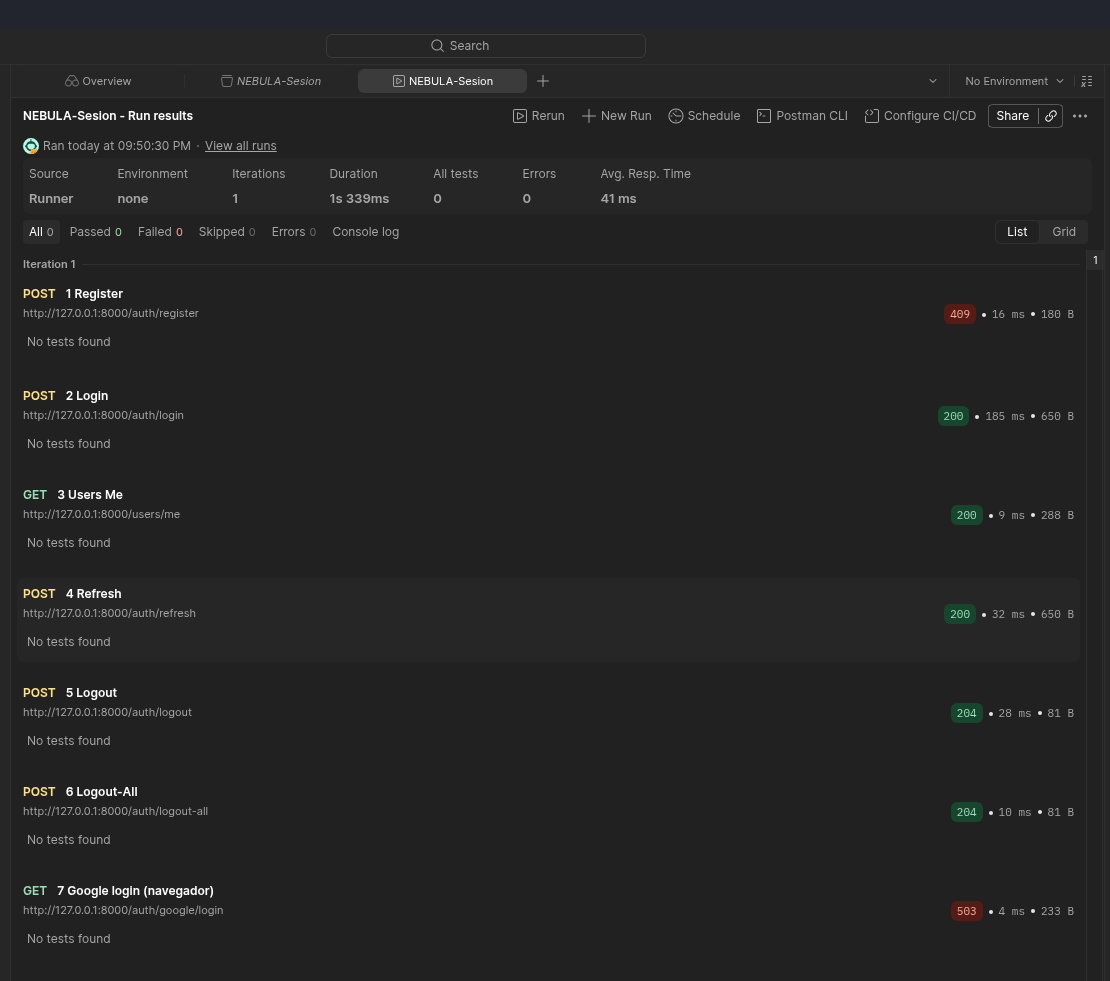
\includegraphics[width=0.95\columnwidth,height=5.5cm,keepaspectratio]{imagenes/16_postman_run_full.png}
    \caption{\footnotesize Postman Runner: full run including 409 on duplicate register and 204 on logout-all (503 on Google login without credentials).}
    \label{fig:postman-run-completo}
\end{figure}

% ------------------------------------------------------------
\subsection{Part 22: Required tests}
\label{sec:verification}

Table~\ref{tab:required-tests} lists the required test cases. The file \texttt{tests/test\_api\_workshop5.py} contains 22 automated tests that use FastAPI's \texttt{TestClient} with a temporary SQLite database. All 22 pass:

\begin{lstlisting}[basicstyle=\ttfamily\footnotesize]
python -m pytest tests/test_api_workshop5.py -v
22 passed
\end{lstlisting}

In addition, the standalone application was started with \texttt{uvicorn} and exercised with \texttt{curl} (root, \texttt{/docs}, register, login, \texttt{/users/me}, 401 without token, 401 with a wrong password, and the stored refresh token), and the modified \texttt{controller.py} compiles. Besides the cases of the workshop, the tests cover reuse of a rotated refresh token, a token signed with another key, a refresh token used as access token (and vice versa), a forged \texttt{user\_id}, dataset/model validation, inactive users and \texttt{logout-all}.

\begin{table}[H]
\centering
\scriptsize
\begin{tabularx}{\columnwidth}{
    >{\raggedright\arraybackslash}X
    >{\raggedright\arraybackslash}X
    >{\raggedright\arraybackslash}X
}
\hline
\textbf{Test} & \textbf{Expected Result} & \textbf{Result} \\
\hline
Public endpoint without JWT & Success & 200 (automated) \\
Registration with valid information & User created & 201, no hash (automated + Fig.~\ref{fig:postman-register-respuesta}) \\
Duplicate email & Rejected & 409 (automated + Fig.~\ref{fig:postman-run-completo}) \\
Invalid email & Rejected & 422 (automated) \\
Login with correct password & Tokens returned & 200, \texttt{expires\_in} 900 (automated + Fig.~\ref{fig:postman-login-respuesta}) \\
Login with incorrect password & 401 Unauthorized & 401 (automated) \\
\texttt{/users/me} without token & Rejected & 401 (automated) \\
\texttt{/users/me} with valid token & User returned & 200 (automated + Fig.~\ref{fig:postman-run-201}) \\
Protected CRUD without JWT & Rejected & 401 (automated) \\
Protected CRUD with JWT & Success & 201 / 200 / 204 (automated) \\
Access another user's protected resource & Rejected & 403 (automated) \\
Expired/invalid token & Rejected & 401 (automated) \\
Refresh valid token & New token issued & 200, rotation (automated + Fig.~\ref{fig:postman-run-201}) \\
Invalid refresh token & Rejected & 401 (automated) \\
Logout & Session/refresh token revoked & 204 (automated + Fig.~\ref{fig:postman-run-201}) \\
Use revoked refresh token & Rejected & 401 (automated) \\
Remember Me = false & Normal refresh lifetime & 7 days (automated) \\
Remember Me = true & Extended refresh lifetime & 30 days (automated) \\
Social registration/login & User authenticated & Social logic automated; unconfigured 503 verified (Fig.~\ref{fig:google-not-configured}); real Google round-trip pending \\
OpenAPI/Swagger test & Success & Specification automated; Swagger UI shown (Fig.~\ref{fig:swagger-docs}); browser run (Fig.~\ref{fig:browser-qa-flow}) \\
Postman test & Success & Collection and Runner (Figs.~\ref{fig:postman-collection}--\ref{fig:postman-run-completo}) \\
\hline
\end{tabularx}
\caption{Required API test cases and results.}
\label{tab:required-tests}
\end{table}

Scope of verification: the 22 automated tests pass; the standalone application was started with \texttt{uvicorn} and exercised with \texttt{curl}; the Postman collection was imported and executed (Figs.~\ref{fig:postman-collection}--\ref{fig:postman-run-completo}); and the browser end-to-end flows were recorded (Figs.~\ref{fig:web-home}--\ref{fig:web-logged-in}, \ref{fig:web-dashboard} and \ref{fig:browser-qa-flow}). Still pending: (1) the real Google round-trip with valid credentials, (2) the Controller running inside Docker on port 5050 (only the wiring of \texttt{include\_api}/\texttt{init\_api} and its compilation were checked), and (3) MySQL/MariaDB or PostgreSQL through \texttt{DATABASE\_URL} (the setting exists, but only SQLite was tested).

% ------------------------------------------------------------
\subsection{Part 23: Minimum endpoint specification}

Table~\ref{tab:min-endpoints} compares the minimum endpoints required by the workshop with the implementation.

\begin{table}[H]
\centering
\scriptsize
\begin{tabularx}{\columnwidth}{>{\raggedright\arraybackslash}X >{\raggedright\arraybackslash}X >{\raggedright\arraybackslash}p{0.22\columnwidth}}
\hline
\textbf{Required endpoint} & \textbf{Implemented} & \textbf{Status} \\
\hline
\texttt{GET /public/info} & \texttt{GET /public/info} & Done \\
\texttt{GET /public/<resource>} & \texttt{/public/datasets}, \texttt{/aggregators}, \texttt{/topologies} & Done \\
\texttt{POST /auth/register} & \texttt{POST /auth/register} & Done \\
\texttt{POST /auth/login} & \texttt{POST /auth/login} & Done \\
\texttt{POST /auth/refresh} & \texttt{POST /auth/refresh} & Done (rotation) \\
\texttt{POST /auth/logout} & \texttt{POST /auth/logout}, \texttt{/auth/logout-all} & Done \\
\texttt{GET /auth/<provider>/login} & \texttt{GET /auth/google/login} & Done; real flow pending \\
\texttt{GET /auth/<provider>/callback} & \texttt{GET /auth/google/callback} & Done; real flow pending \\
\texttt{GET /users/me} & \texttt{GET /users/me} & Done \\
\texttt{POST /<entities>} & \texttt{POST /experiments} & Done \\
\texttt{GET /<entities>} & \texttt{GET /experiments} & Done \\
\texttt{GET /<entities>/\{id\}} & \texttt{GET /experiments/\{id\}} & Done \\
\texttt{PUT /<entities>/\{id\}} & \texttt{PUT /experiments/\{id\}} & Done (+ \texttt{PATCH}) \\
\texttt{DELETE /<entities>/\{id\}} & \texttt{DELETE /experiments/\{id\}} & Done \\
\hline
\end{tabularx}
\caption{Minimum endpoint specification versus the implementation.}
\label{tab:min-endpoints}
\end{table}

% ------------------------------------------------------------
\subsection{Part 24: Security requirements}

\begin{table}[H]
\centering
\small
\begin{tabularx}{\columnwidth}{X l X}
\hline
\textbf{Requirement} & \textbf{Status} & \textbf{Notes} \\
\hline
Never store plain-text passwords & Met & Argon2id; \texttt{NULL} for social accounts \\
Never return password hashes & Met (API) & \texttt{UserResponse} has no hash. The legacy Controller route \texttt{/user/list?all\_info=true} still returns them \\
Keep secrets outside the source code & Met (API) & \texttt{JWT\_SECRET} and Google credentials from the environment; the app fails without \texttt{JWT\_SECRET}. The Firebase web configuration remains in \texttt{layout.html} \\
Do not commit \texttt{.env} & Met & In \texttt{.gitignore}, as are the \texttt{api.db} files; \texttt{.env.example} has no real values \\
Validate JWT signature and expiration & Met & \texttt{decode\_token}; tested with an expired token and a token signed with another key \\
Distinguish access and refresh tokens & Met & \texttt{type} claim; tested in both directions \\
Revoke refresh tokens on logout & Met & \texttt{revoked\_at}, rotation, reuse detection, \texttt{logout-all} \\
Validate ownership before modifying resources & Met & \texttt{get\_owned\_experiment}; tested for GET, PUT, PATCH, DELETE \\
Validate request data with Pydantic & Met (API) & Constrained fields, \texttt{EmailStr}, \texttt{Literal}, dataset/model validator. The SMAC web endpoints still read \texttt{request.json()} \\
Do not trust client-supplied identity & Met (API) & Owner taken from the JWT; OAuth exchange completed on the server. The Firebase web login still trusts the browser \\
Use HTTPS & Not met & Local deployment uses HTTP; behind a TLS proxy and with \texttt{NEBULA\_PRODUCTION=True}, the OAuth cookie becomes \texttt{https\_only} \\
\hline
\end{tabularx}
\caption{Compliance with the workshop security requirements.}
\label{tab:security}
\end{table}

\paragraph{Known limitations.}
\begin{itemize}
    \item The existing Controller routes (\texttt{/user/add}, \texttt{/user/delete}, \texttt{/user/update}, \texttt{/scenarios/run}, \texttt{/scenarios/stop}, \texttt{/physical/...}) have no authentication, and the deployer publishes the Controller port. They were not protected because the NEBULA frontend calls them without a token and doing so would break the platform. Possible solutions are a service token for the frontend or not exposing port 5050 outside the Docker network.
    \item There is no rate limiting or lockout on \texttt{/auth/login}.
    \item There is no denylist for access tokens; a stolen access token is valid for up to 15 minutes even after logout.
    \item Expired and revoked refresh tokens are not purged periodically.
    \item The tables are created with \texttt{create\_all}; production use should adopt migrations (Alembic).
    \item The most important pending fix of the web application is to verify the Firebase ID token on the server (for example with \texttt{firebase\_admin.auth.verify\_id\_token}) and to stop assigning the fixed password \texttt{firebase\_auth} to Google accounts.
\end{itemize}

% ------------------------------------------------------------
\subsection{Part 25: Final API workflow}

The REST API supports the workflow of the workshop:

\begin{enumerate}
    \item \textbf{Register}: \texttt{POST /auth/register} creates a local account with role \texttt{user}.
    \item \textbf{Login}: \texttt{POST /auth/login} validates the credentials and returns an access token (15 minutes) and a refresh token (7 or 30 days), which is registered in the database.
    \item \textbf{Protected CRUD}: with \texttt{Authorization: Bearer <access-token>}, the user manages their own experiments.
    \item \textbf{Access token expires}: protected endpoints answer 401.
    \item \textbf{Refresh}: \texttt{POST /auth/refresh} revokes the used refresh token and returns a new pair.
    \item \textbf{Protected CRUD} again with the new access token.
    \item \textbf{Logout}: \texttt{POST /auth/logout} revokes the refresh token; using it again returns 401.
\end{enumerate}

The alternative authentication path is: Google $\rightarrow$ OAuth 2.0 / OIDC $\rightarrow$ \texttt{GET /auth/google/callback} $\rightarrow$ create or find the user $\rightarrow$ application JWTs $\rightarrow$ protected API.

The NEBULA web application (port 6060) keeps its own session-cookie authentication, which supports registration, login, Firebase Google sign-in, logout and the SMAC functionality. Both mechanisms coexist: the web interface uses the session, and the REST API uses JWT. Figure~\ref{fig:web-dashboard} shows the dashboard of the QA account after the browser login, ready to deploy a scenario.

\begin{figure}[H]
    \centering
    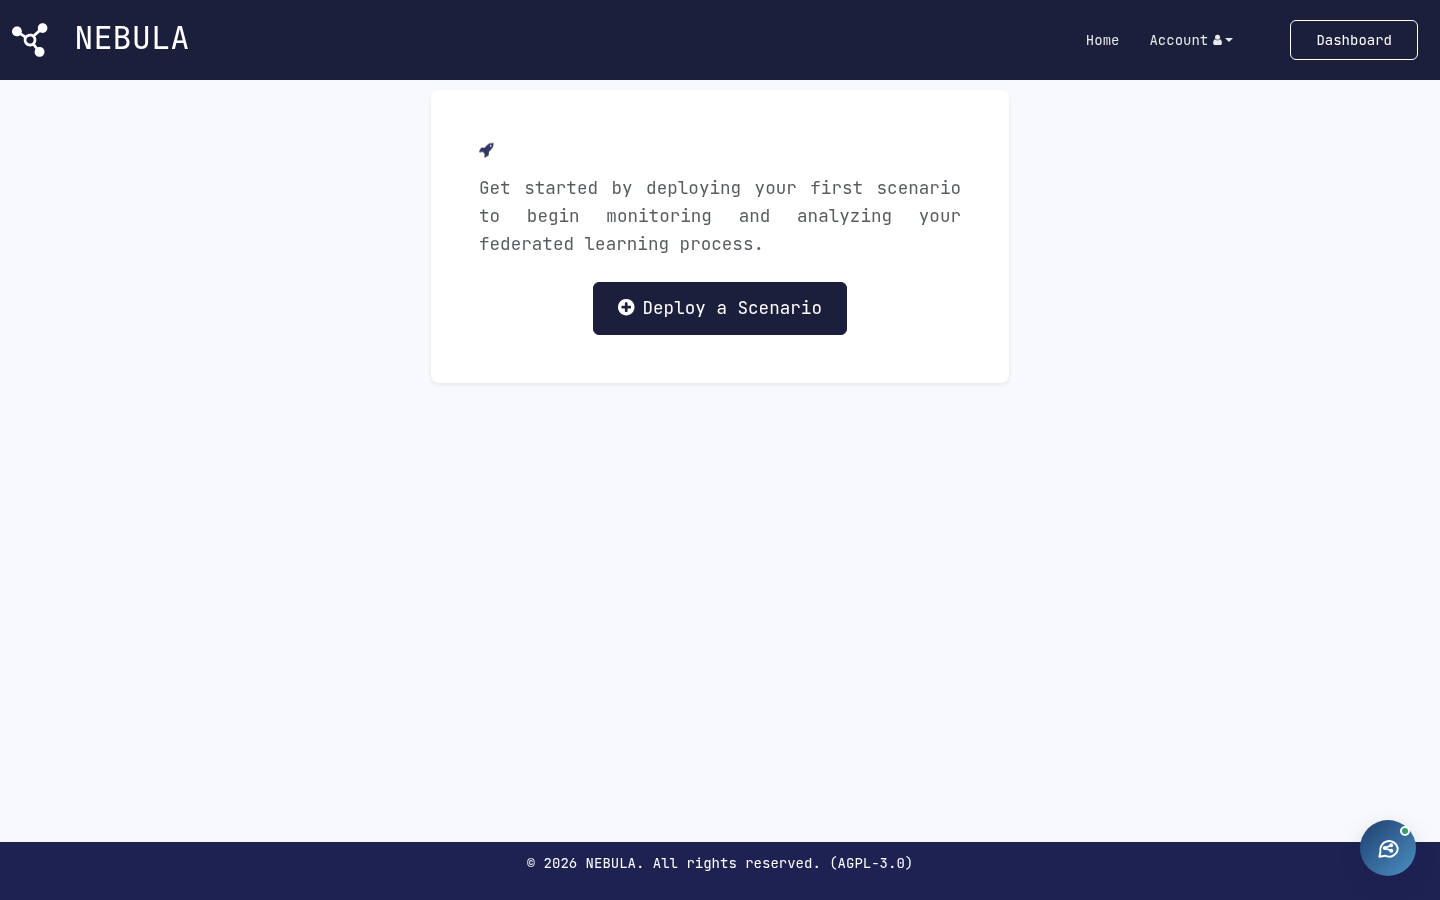
\includegraphics[width=0.95\columnwidth,height=5.5cm,keepaspectratio]{imagenes/17_web_dashboard.png}
    \caption{\footnotesize Dashboard of the QA account after the browser login.}
    \label{fig:web-dashboard}
\end{figure}




\bibliographystyle{IEEEtran}
\bibliography{ref}


\end{document}
